\documentclass[withoutpreface,bwprint]{cumcmthesis} %去掉封面与编号页,电子版提交的时候使用。


\renewcommand\thepage{\zihao{-4} ~\arabic{page}~}%字体宋体,字号小四
\linespread{1}%1倍行距
\usepackage{booktabs}%三线表必备
\usepackage{appendix}
% 其他奇怪的包
% Useful packages
\usepackage{amsmath}
\usepackage{graphicx}
\usepackage{listings}
\usepackage{float}
\usepackage{makeidx}
\usepackage[utf8]{inputenc}
\usepackage{array}
\usepackage{multirow}
\usepackage{caption}   % 图片脚注
\usepackage{caption}
\usepackage{subfigure} % 子图包
\newcommand\MyBox[2]{
  \fbox{\lower0.75cm
    \vbox to 1.7cm{\vfil
      \hbox to 1.7cm{\hfil\parbox{1.4cm}{#1\\#2}\hfil}
      \vfil}%
  }%
}


\title{\heiti \zihao{3}基于整数规划与概率分布的最优核酸混检方案}
\tihao{A}
\baominghao{43}
\schoolname{复旦大学、Columbia University}
\membera{孙夏炀}
\memberb{任逸昂}
\memberc{陆天一}
\supervisor{蔡志杰、李传峰}
\yearinput{2022}
\monthinput{05}
\dayinput{01}

\begin{document}

\maketitle
\begin{abstract}

为提高效率节省资源,在大规模进行核酸检测筛查新冠感染者时,应根据情况合理设计混合检测策略。

\textbf{对于问题一:}
在模型一中,首先根据检测资源情况不同分成“充足”、“相对不足”、“严重不足”分类讨论。对第一类,基于各区每天的感染建立\textbf{总检测次数与各区混检数的函数关系},并求其最小值与相应的混检数;对另两类情况,将这个区检测数分类“\textbf{混检数}”和“\textbf{复检数}”,借助各区阳性率的差异调配最大检测数至各区从而查出尽可能多的感染者,建立\textbf{总检测次数}、\textbf{混检数}、\textbf{复检数}之间的约束条件,利用\textbf{分支界定法}求解以上变量的最优解,从而得到最优混检方案。 

针对模型一中情况一,我们将混淆矩阵、混检的稀释作用等纳入考量,建立了模型二。模型二中使用\textbf{各区诊断某一人感染情况所需检测次数的期望}与各区混检样本数的函数关系,并运用枚举法求其最小值与相应的混检样本数。\\

\textbf{对于问题二:} 
收集了美国纽约2022年1月26日至4月26日5个辖区每日新冠检测阳性率数据,代入问题一中所建模型给出各区每日混检样本数最优方案。约定纽约市检测资源充足。根据各区每日阳性率不同,各区最优混检方案为5$\sim$14人一组。以美国纽约市Brooklyn地区为例(2022年1月31日检测阳性率为5.02\%),计算得出\textbf{最佳混检样本大小为6,平均每人检测量为0.5161,最少需要检测1321421次}。\\

\textbf{对于问题三:} 
多轮混检用于处于潜伏期未被查明的阳性感染者。数据分析发现其服从$ \chi^2  \left(3.5\right)$分布\cite{wuhan},借助已测得感染率,基于假设的潜伏期分布推得实际感染率$\rho^*$,并以此数据带入问题一的两个模型中求解相应混检样本大小。真实阳性率略大于检测阳性率,推断得出根据实际情况得出的混检策略大体相同,以美国纽约市Manhattan地区为例(2022年2月15日的预测感染率为2.20\%),此时模型给出\textbf{最佳混检样本大小为8},\textbf{最少检测次数为446265次}。\\
\thispagestyle{empty}
\end{abstract}

\setcounter{page}{1}
\section{问题重述}
2019 年底、2020 年初开始席卷全球的新冠疫情,给人类的生命安全带来了极
大的威胁。为了有效控制新冠病毒的传播,核酸检测是一个非常重要而有效的手
段。核酸检测需要一定的时间,在进行大规模核酸检测时,往往会因为来不及检测
而耽误控制病毒传播的宝贵时间。为此,通常采用混合检测的方法,将若干人组成
一组,把他们的采样样本混合起来一起进行检测,以加快总体检测速度。如果一组
样本检测结果为阴性,那么这组样本对应的被检测者都是阴性的。如果一组样本检
测结果为阳性,那么这组样本中至少有 1 人是阳性的,需要对这组样本的所有被检
测者重新进行检测。重新检测时,采用单人单管检测的方法,以确定哪一个或哪几
个被检测者是阳性的。

 \begin{problem}
请建立数学模型,分析说明多少人一组进行混检是比较理想的。。
 \end{problem}
 \begin{problem}
收集相关数据,利用问题 1 的数学模型给出相应的混检方案。
 \end{problem}
 \begin{problem}
在出现疫情时,通常需要进行多轮检测。请利用建立的数学模型说明,
在多轮检测中,是否需要调整混检方案。如果需要调整方案,如何进行调整。
\end{problem}

\section{问题分析}
\subsection{问题一分析}
针对问题一,建立了两个模型探讨多少人一组进行混检是比较理想的。
在模型一中,讨论了在新冠检测能力充足、有限及严重不足的不同条件下的最佳混检策略。为此,在固定阳性率下,建立了非线性整数规划模型来探讨混检样本数量对最终检测总数与测得阳性量期望的关系。并运用牛顿迭代法求得其数值解。
在模型二中,进一步将核酸检测错误率、混检的稀释作用等纳入考量,构造混淆矩阵,将诊断某一人感染情况所需检测次数的期望值作为最优混检策略的评价指标。并运用枚举法根据各地区各时间不同阳性率得到相应的不同的混检策略。

\subsection{问题二分析}
针对问题二,我们首先应寻找恰当的样本,随后利用问题一中给出的模型求解最优的混检策略。在问题一给出的两种模型中与待检测样本相关的参数仅有平均阳性率。因此,我们找到了美国纽约市2022年1月26日至4月26日各区新冠检测阳性率数据作为样本。当地政府目前并没有疫情管制措施,但很多公司要求员工定期进行新冠检测。一些大学,例如哥伦比亚大学,更有每周随机抽检学生调研阳性率的要求\cite{columbia}。故该数据可以作为当地新冠病毒的平均感染率之合理估计。将这些数据代入建立的两个模型即可得出对应条件下建议混检方案。

\subsection{问题三分析}
针对问题三,我们首先需明白多轮混检的本质意义,即:发现在过去的检测中由于处于潜伏期未被查明的阳性感染者。由于我们得到的数据仅记录每日查明的感染者,因此实际的感染率比记录的数据高。故我们进一步分布运用概率分布对“每日实际的感染率”建模,得到当日实际的感染率关于之前数日的实际的感染率的递推公式并求解。随后将该数据替换掉模型一、二中的参数“感染率”,重新求解多轮混检的最优混检策略,并将新的结果与原结果进行比较,从而得到两者的差异。
\section{模型假设}
\begin{enumerate}
    \item 假设单只采样管最大收集样本数为32\cite{max_maps};
    \item 假设某地区根据行政规划可划分为不同区域,区域间的感染者数是独立的;
    \item 忽略各个地区阳性感染者分布不均产生的影响;
    \item 忽略核酸检测速度。
\end{enumerate}

\section{符号说明}
\begin{table}[H] %开始table相关的指令
    \begin{center} %整个表格居中
    \caption{符号说明} %将该表格命名为#(与下面的#没关系)
    \begin{tabular}{cl} %开始进行表格部分的设置
    %此处表格有几列就有几个#,此处以两列为例
    %其中#可以是l,c,r(分别表示该列中所有元素居左,中,右)
        \toprule %设置顶线,接下来设置表格的内容
        \multicolumn{1}{m{3cm}}{\centering 符号} %赋予从左往右数的一列以第一等级的标题A
        & \multicolumn{1}{m{10cm}}{ 含义} %这里表示紧接着前面的那一列的接下来三列合并并规定长度为六厘米
        \\ %换行开始定义表格具体内容
        \midrule %赋予第一等级的中线
        $\Omega_k$	&第$k$个区域\\
        $x_k$  &地区$\Omega_k$混检混合样本量\\
        $\rho_k(t)$	&第$t$天地区$\Omega_k$的新冠平均感染率\\
        $\rho^*_k(t)$ &第$t$天地区$\Omega_k$的(考虑潜伏期后)实际新冠平均感染率 \\
        %$\rho_k$    &对$\rho_k(t)$的缩写(模型2) \\
        %$\rho_e$	&混检异常的情况下复检阳性的平均感染率\\
        $n_k$       &地区$\Omega_k$混检样本的大小(人口数)\\
        $w_0$       &最大检测量\\
        $w$	        &检测能力充足时最小检测数\\
        %$w_k$       &地区$\Omega_k$的混检量与复检量的总和 \\
        %$u_k$       &地区$\Omega_k$的混检量\\
        %$v_k$       &地区$\Omega_k$的复检量\\
        $z$         &所有地区单日复检阳性人数的总和\\
        $TPR'$      &考虑混检稀释作用后的真阳性占感染者总人数之比 \\
        $TNR$       &真阴性占非感染者总人数之比 \\
        $S_k(x_k)$    &诊断地区$\Omega_k$中某一人感染情况所需检测次数 \\
         \bottomrule
        \end{tabular} \label{tb:符号说明}%结束表格内容部分设置并赋予该部分内容以标签tb:notations
    \end{center} %结束整体居中处理部分的定义
\end{table} %结束table相关的指令


\section{问题一模型建立与求解}

\subsection{模型一建立}
假设某地区根据某种规则可划分为$N$个区域:$\{\Omega_k \vert 1\leq k \leq N \}$;
假设对诸区域$\Omega_k$,其人口数为$n_k$;

假设对诸区域$\Omega_k$,施行$x_k$人一组混合检测(若$x_k$不是$n_k$的因数,对$\dfrac{n_k}{x_k}$作向上取整);

假设对诸区域$\Omega_k$,第$t$天平均阳性率为$\rho_k(t)$,那么对诸区域在一组人中存在阳性的平均概率为:$1-(1-\rho_k(t))^{x_k}$,即对于每组人复检数量期望为:$(1-(1-\rho_k(t))^{x_k})x_k$,那么在整个样本中,复检数量期望为:$n_k(1-(1-\rho_k(t))^{x_k})$。

首先如果不考虑检测资源体量有限的要求,此假设下我们要使检测数达到最少。然而实际上故当疫情社会面扩散时在无增援的情况下,单日最大检测量往往不能满足所需检测量,因此我们需要对检测资源的分配进行决策。事实上不同地区阳性率分布不均,阳性感染者增长率也不同,所以决策时应视地区的严重程度分配不同的资源,应将更多的检测资源,特别是复检的资源放在感染者增长率高的地区,才能更有效得筛出阳性感染者,阻断疫情传播。

\textbf{因此我们所需求解的最优解决方包括:}
\begin{itemize}
    \item 当检测资源充足时,求不同地区最优的混检混合样本数$x_k$,使得混检与复检$w$总检测次数最少;
    \item 当检测资源严重不足时,求不同地区最优的混检混合样本数$x_k$,以及每天分配在诸地区的混检量$u_k$与复检量$v_k$,使得所有地区当天能筛查出阳性感染者总数$z$最多;
    \item 当检测资源相对不足时,求不同地区最优的混检混合样本数$x_k$,以及每天分配在诸地区的混检量$u_k$与复检量$v_k$,使得所有地区在保证全员做一次混检的前提下,使得当天能筛查出阳性感染者总数$z$最多。
\end{itemize}

进一步,假设可用的最大检测量为$w_0$;

假设诸$w_k$的混检量分配到诸$\Omega_k$的混检量为$u_{k}$,混检后复检量为$v_{k}$,两者之和为最大检测量$w_0$,即:
\begin{align}
    w_0 \geqslant \sum^N_{k=1} u_k +\sum^N_{k=1} v_k
\end{align}

假设异常采样管的平均阳性率为$\rho_{e}$,

一方面,只有先混检才能复检,复检量不得超过混检异常管中的样本总和,否则会造成浪费,当不再出现新增感染者时也不会做复检,即:
\begin{align}
    v_k &\leqslant {\rm max} \{0, n_k\cdot(1-(1-\rho_k(t))^{x_k})-(1-(1-\rho_k(t-1))^{x_k}) \}\\
    \Rightarrow v_k &\leqslant n_k \cdot {\rm max} \{0, (1-\rho_k(t-1))^{x_k}-(1-\rho_k(t))^{x_k}\}
\end{align}

另一方面,只有复检可以确定阳性感染者,我们要使每轮检测可以查出的新增阳性感染者数目最多,即:
\begin{equation}
    {\rm max} \quad \sum^N_{k=1}\rho_e v_k
\end{equation}


于是问题转化为求诸$u_k,v_k(k=1,2,...,N)$,和$x$,s.t.:
\begin{itemize}
    \item{1.}
    当$w_0 \geqslant \sum\limits^N_{k=1}\dfrac{n_k}{x_k} + \sum\limits^N_{k=1}n_k  (1-(1-\rho_k(t))^{x_k})$,即检测能力充足时:
\begin{align}
\label{naive}
    {\rm min} \quad w= \sum^N_{k=1} \frac{n_k}{x_k}+ n_k\cdot {\rm max} \left\{0,(1-\rho_k(t-1))^{x_k}-(1-\rho_k(t))^{x_k}\right\}
\end{align}
    
    \item{2.}
        当$\sum\limits^N_{k=1}\dfrac{n_k}{x_k} \leqslant w_0 \leqslant\ \sum\limits^N_{k=1}\dfrac{n_k}{x_k} + \sum\limits^N_{k=1}n_k  (1-(1-\rho_k(t))^{x_k})$,即检测能力相对不足时:
\begin{align}
\label{eq2}
    \left\{
    \begin{aligned}
        &x_k \geqslant 2 \\
        &u_k =\frac{n_k}{x_k} \\
        &0 \leqslant v_k \leqslant  n_k \cdot {\rm max}
         \{0,(1-\rho_k(t-1))^{x_k}-(1-\rho_k(t))^{x_k} \} \\
        &{\rm max} \quad z = \sum^N_{k=1}\rho_e v_k  \\
        &w_0 \geqslant \sum^N_{k=1} u_k +\sum^N_{k=1} v_k  \\
        &u_k,v_k,x_k\in\mathbb{Z^+}\\
        &k=1,2,...,N \\
    \end{aligned}
    \right.
\end{align}

    \item{3.}
当$w_0 < \sum\limits^N_{k=1}\dfrac{n_k}{x_k}$,即检测能力严重不足时:
\begin{align}
\label{eq3}
    \left\{
    \begin{aligned}
        &x_k \geqslant 2  \\
        &u_k \geqslant 0  \\
        &0\leqslant v_k \leqslant u_k \cdot x_k \cdot {\rm max} \{0,(1-\rho_k(t-1))^{x_k}-(1-\rho_k(t))^{x_k} \} \\
        &w_0 \geqslant \sum^N_{k=1} u_k +\sum^N_{k=1} v_k  \\
        &{\rm max} \quad z = \sum^N_{k=1}\rho_{e} v_k  \\
        &u_k,v_k,x_k\in\mathbb{Z^+}\\
        &k=1,2,...,N \\
    \end{aligned}
    \right.
\end{align}
    


\end{itemize}


\subsection{模型一求解准备}
\subsubsection{牛顿法}
牛顿法(Newton's method)是一种在实数域和复数域上近似求解方程的方法。方法使用函数$f(x)$的泰勒级数的前面几项来寻找方程$f(x)=0$的根。
首先,选择一个接近函数$f(x)$零点的$x_{0}$,计算相应的$f(x_0)$和切线斜率$f'(x_0)$。然后我们计算穿过点$(x_0,f(x_0))$并且斜率为$f'(x_0)$的直线和$x$轴的交点的$x$坐标,也就是求如下方程的解:
\begin{align*}
    &0=(x-x_0)\cdot f'(x_0)+f(x_0)
\end{align*}
我们将新求得的点的x坐标命名为$x_1$,通常$x_1$会比$x_0$更接近方程$f(x)=0$的解。因此我们现在可以利用$x_1$开始下一轮迭代。迭代公式可化简为如下所示:
\begin{align*}
    &x_{n+1}=x_n-\frac{f(x_n)}{f'(x_n)}
\end{align*}

\subsubsection{分支界定法}
分支定界法的求解步骤为:
\begin{itemize}
    \item 第一步: 求整数规划的松弛问题最优解;若松弛问题的最优解满足整数要求,得到数规划的最优解,否则转下一步;
    
    \item 第二步: 分支与定界:任意选一个非整数解的变量$x_i$,在松弛问题中加上约束:$x_i≤[x_i]$ 和 $x_i≥[x_i]+1$组成两个新的松弛问题,称为分枝。
    
    \item 第三步: 剪枝: 检查所有分枝的解及目标函数值,若某分枝的解是整数并且目标函数值大于(max)等于其它分枝的目标值,则将其它分枝剪去不再计算,若还存在非整数解并且目标值大于(max)整数解的目标值,需要继续分枝,再检查,直到得到最优解。
\end{itemize}

\subsection{模型一求解}
\subsubsection{第一种情况}
先考虑检测资源充足的情况,求解优化问题\ref{naive},需对式\ref{naive}中代数式对诸$x_k$求偏导,建立一阶条件(FOC),即:
\begin{align*}
w_k = \dfrac{\partial}{\partial x_k} \left( \sum^N_{i=1} \frac{n_i}{x_i}+ n_k\cdot   ((1-\rho_i(t-1))^{x_i}-(1-\rho_i(t))^{x_i}) \right),\quad k=1,2,...,N
\end{align*}
化简得:
\begin{align}
\label{naive_sol}
\left\{
\begin{aligned}
        &\forall k \leqslant N,(1-\rho_k(t-1))^{x_k}\ln(1-\rho_k(t-1))-(1-\rho_k(t))^{x_k}\ln(1-\rho_k(t))=\frac{1}{x^2_k}; \\
    &w=\sum^N_{k=1}w_k.
\end{aligned}
\right.
\end{align}


该方程为超越方程,难以求得解析解,故使用牛顿法求取数值解。

由于方程组\ref{naive_sol}中每个方程是独立的,不妨取$N=1$进行结果展示
\begin{figure}[H]
\centering
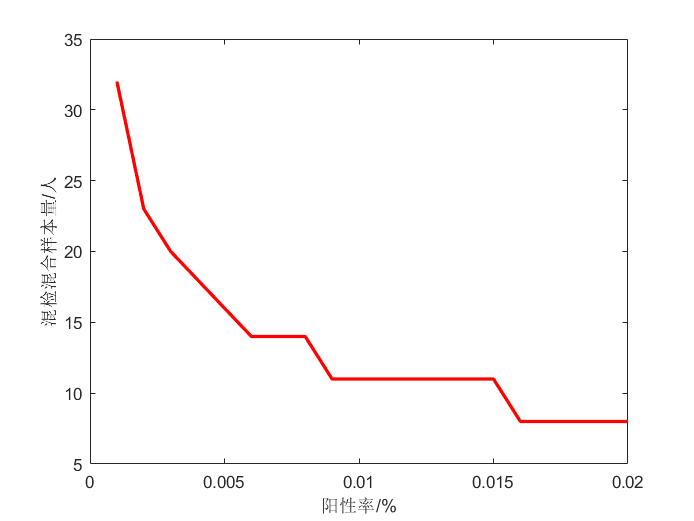
\includegraphics[width=0.5\textwidth]{fig_pro1.png}
\caption{不同阳性率下,推荐混检混合样本量}
\label{pro1}
\end{figure}

如上图所示,曲线展示了最优混检混合样本数随某地区平均阳性率的变化关系的一个例子:取定$\rho_k(t-1)=0$,取横坐标为$\rho_k(t)$,纵坐标为最优混检混合样本$x$.可以看到$x$随$\rho_k(t)$的增大而减小.当$\rho_k(t)<0.5\%$时,病毒感染率极低,单管样本数过少则资源浪费过大,因此$x$可取的较大;当$\rho_k(t) \geqslant 0.5\%$时,病毒感染率增大,则需开始削减单管样本数;同时当$x$取10附近的值时,$\rho_k(t)$的取值也约在$0.1\% \sim 0.15\%$,此即2022年上海疫情中新冠病毒奥密克戎变种的阳性感染率,因此模型结果是符合事实的

\subsubsection{第二种情况}
对于方程\ref{eq2},显然要使得$z$最大,则$v_k$需尽可能大,此时方程\ref{eq2}中的不等式均取边界条件,得到:
\begin{align}
\label{eq2solution1}
    \left\{
    \begin{aligned}
        &u_k =\dfrac{n_k}{x_k} \\
        &v_k =n_k \cdot {\rm max}
         \{0,(1-\rho_k(t-1))^{x_k}-(1-\rho_k(t))^{x_k} \} \\
        &{\rm max} \quad z = \sum^N_{k=1}\rho_e v_k  \\
        &w_0 =\sum^N_{k=1} u_k +\sum^N_{k=1} v_k  \\
        &u_k,v_k,x_k\in\mathbb{Z^+},\quad  x_k \geqslant 2  \\
    \end{aligned}
    \right.
\end{align}
将第二个式子中的$v_k$代入第一个和第三个式子得到
\begin{align}
\label{eq2solution1}
\quad\left\{
    \begin{aligned}
        &max\quad z = \sum^N_{k=1}\rho_e n_k \cdot {\rm max}
         \{0,(1-\rho_k(t-1))^{x_k} - (1-\rho_k(t))^{x_k} \}   \\
        &w_0 = \sum^N_{k=1} u_k\cdot {\rm max} \{1, n_k  [(1-\rho_k(t-1))^{x_k}-(1-\rho_k(t))^{x_k}] +1 \} \\
        &u_k,x\in\mathbb{Z^+}, \quad x_k \geqslant 2 \\
    \end{aligned}
    \right.
\end{align}
令$f_k(x) = (1-\rho_k(t-1))^{x_k}-(1-\rho_k(t))^{x_k}$,则上式可化简为
\begin{align}
\label{eq2solution1}
\quad\left\{
    \begin{aligned}
        &max\quad z = \sum^N_{k=1}\rho_e u_k f_k(x)  \\
        &w_0 = \sum^N_{k=1} u_k \cdot {\rm max}\{1,f_k(x)+1\}  \\
        &u_k,x\in\mathbb{Z^+},  \quad x_k \geqslant 2 \\
    \end{aligned}
    \right.
\end{align}

如果将诸$x_k$固定,则此问题化为整数线性规划问题,可使用分支定界法求解\cite{bib20}。

取$N=2,w_0=3000,\rho_1(t-1)=0=\rho_2(t-1)=0,\rho_1(t)=0.01,\rho_2(t)=0.02$,解得:
\begin{align*}
    u_1=v_1=0, u_2=\dfrac{w_0}{x_2},v_2=w_0-u_2
\end{align*}
由于$u_1=v_1=0$,故$x_1$不起作用,作$z$随$x_2$的变化曲线如图所示:
\begin{figure}[H]
\centering
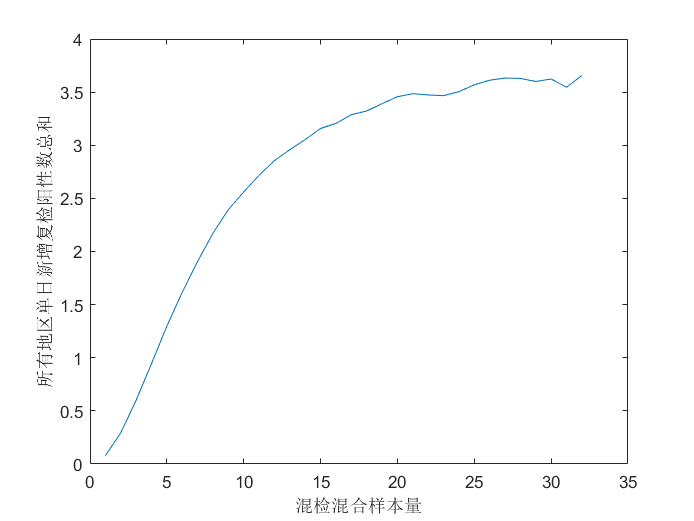
\includegraphics[width=0.5\textwidth]{fig_pro2.png}
\caption{阳性率给定,推荐混检混合样本量}
\label{pro1}
\end{figure}

单日复检阳性人数的总和$z$与混检样本数$x$成正相关,即当资源严重不足时要使单日检测出的阳性人数最多,首先尽可能将资源安排给感染增长率快的地区,其次在该地区内单只采样管的样本数取上限32即可。

但是,在$x$取到12附近时,曲线的斜率开始递减,即每日新增感染者的增长率虽$x$放缓,从这个角度出发,同样尽可能将资源安排给感染增长率快的地区,但在在该地区内单只采样管的样本数取12即可。

\subsubsection{第三种情况}
对于方程\ref{eq3},显然要使得$z$最大,则$v_k$需尽可能大,此时方程\ref{eq3}中的不等式均取边界条件,得到:
\begin{align}
\label{eq2solution1}
    \left\{
    \begin{aligned}
        &u_k \geqslant 0 \\
        &v_k =u_k x_k\cdot {\rm max}
         \{0,(1-\rho_k(t-1))^{x_k}-(1-\rho_k(t))^{x_k} \} \\
        &{\rm max} \quad z = \sum^N_{k=1}\rho_e v_k  \\
        &w_0 =\sum^N_{k=1} u_k +\sum^N_{k=1} v_k  \\
        &u_k,v_k,x_k\in\mathbb{Z^+}, \quad x_k \geqslant 2\\
    \end{aligned}
    \right.
\end{align}

将第二个式子中的$v_k$代入第一个和第三个式子得到
\begin{align}
\label{eq2solution1}
\quad\left\{
    \begin{aligned}
        &max\quad z = \sum^N_{k=1}\rho_e u_k x_k \cdot {\rm max}
         \{0,(1-\rho_k(t-1))^{x_k}-(1-\rho_k(t))^{x_k} \}   \\
        &w_0 = \sum^N_{k=1} u_k\cdot {\rm max} \{1, u_k x_k  [(1-\rho_k(t-1))^{x_k}-(1-\rho_k(t))^{x_k}] +1 \} \\
        &u_k,x\in\mathbb{Z^+}\\
    \end{aligned}
    \right.
\end{align}

令$f_k(x) = (1-\rho_k(t-1))^x-(1-\rho_k(t))^x)x$,则上式可化简为
\begin{align}
\label{eq2solution1}
\quad\left\{
    \begin{aligned}
        &max\quad z = \sum^N_{k=1}\rho_e u_k f_k(x)  \\
        &w_0 = \sum^N_{k=1} u_k \cdot {\rm max}\{1,f_k(x)+1\}  \\
        &u_k,x_k\in\mathbb{Z^+} \quad x_k \geqslant 2 \\
    \end{aligned}
    \right.
\end{align}

如果将$x_k$固定,则此问题化为整数线性规划问题,可使用分支定界法求解\cite{bib20}。

取$N=2,w_0=3000,\rho_1(t-1)=0=\rho_2(t-1)=0,\rho_1(t)=0.01,\rho_2(t)=0.02$,解得:
\begin{align*}
    u_1=v_1=0, u_2=\dfrac{w_0}{x_2},v_2=w_0-u_2
\end{align*}
由于$u_1=v_1=0$,故$x_1$不起作用,作$z$随$x_2$的变化曲线如图所示:
\begin{figure}[H]
\centering
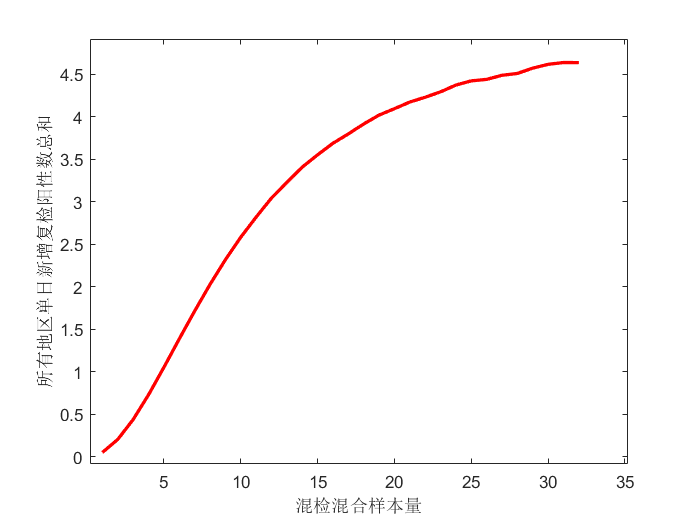
\includegraphics[width=0.5\textwidth]{fig_pro3.png}
\caption{阳性率给定,推荐混检混合样本量}
\label{pro1}
\end{figure}

所有地区单日复检阳性人数的总和$z$与混检样本数$x$成正相关,即当资源严重不足时要使单日检测出的阳性人数最多,首先尽可能将资源安排给感染增长率快的地区,其次在该地区内单只采样管的样本数取上限32即可。

但是,在$x$取到17附近时,曲线的斜率开始递减,即每日新增感染者的增长率虽$x$放缓,从这个角度出发,同样尽可能将资源安排给感染增长率快的地区,但在在该地区内单只采样管的样本数取17即可。

2022年上海疫情爆发初期仍实行网格化管理,检测需求低故资源相对充足,只在重点区域开展核酸检测并施行从10人一管至20人一管不等的混检,在有限的能力下尽最大可能得定位阳性感染者。

\subsection{模型二建立}
对于模型一中的情况1,由于检测资源充足因此我们可以对资源分配进一步细分总而进一步减少检测总数,同时考虑真假阴阳性各自的概率(混淆矩阵),从统计平均的角度给出决策.

%假设复检时核酸绝对准确反映感染情况。

假设对诸区域$\Omega_k$,平均阳性率为$\rho_k$;

该地区施行$x_k$人一组混合检测(若$x_k$不是$n_k$的因数,对$\dfrac{n_k}{x_k}$作向上取整);

假设核酸并非完全准确,即可能存在真阳性(TP)、假阴性(FN)、假阳性(FP)、真阴性(TN)四种情况,其对应的概率分别为$P_{TP},P_{FN},P_{FP},P_{TN}$.令检测结果阳性的感染者与所有感染者人数之比为$TPR$ (Positive Predictive Value, aka. Sensitivity),检测结果阴性的非感染者与所有非感染者之比为$TNR$ (True Negative Rate, aka. Specificity),得到:

\begin{align}
\label{TPR}
    TPR=\dfrac{P_{TP}}{P_{TP}+P_{FN}};  \\
    TNR=\dfrac{P_{TN}}{P_{TN}+P_{FP}};  
\end{align}

% citation to be added
C.D. Pilcher et al (2020)\cite{bib1}指出,在混检核酸时TPR会随着混检池$x_k$增大而降低至$TPR_k$。根据其研究,具体对应关系为:
\begin{align}
    TPR_k=TPR\cdot (1-\dfrac{\log_{10}x_k}{7})
\end{align}
进一步,简记:$\rho_k =\rho_k(t)$,计算混测时的$P_{TP},P_{FN},P_{FP},P_{TN}$得:
\begin{align}
    P_{TP}&=(1-(1-\rho_k)^{x_k})\cdot TPR_k\\
    P_{FP}&=(1-\rho_k)^{x_k}\cdot(1-TPR_k)\\
    P_{TN}&=(1-\rho_k)^{x_k}\cdot TNR\\
    P_{FN}&=(1-(1-\rho_k)^{x_k})\cdot (1-TNR)
    \label{FN}
\end{align}


选择\textbf{诊断某一人感染情况所需检测次数}作为标准来评价每种分组策略。显然,该指标越小,核酸检测的总体速度越快,决策越优。

设地区$\Omega_k$诊断某一人感染情况所需检测次数为$S_{k}(x_k)$

不失一般性,地区$\Omega_k$共需要做$ \dfrac{n_k}{x_k}$ 次混检 ,则地区$\Omega_k$第$j$批人$(k\leqslant N,1 \leqslant j \leqslant \dfrac{n_k}{x_k})$诊断某一人感染情况所需检测次数为$S_{kj}(x_k)$,于是:
%设某一组混合检测$\omega_{kj}$。可得

\begin{align}
\label{skj}
    S_{kj}(x_k)=\left\{
    \begin{aligned}
        &\dfrac{x_k+1}{x_k},&TP\: or\: FP\\
        &\dfrac{1}{x_k},&TN\: or\: FN\\
    \end{aligned}
    \right.
\end{align}

可计算$ S_{kj}(x_k)$的期望为:
\begin{align*}
    E[S_{kj}(x_k)]=\dfrac{x_k+1}{x_k}\cdot (P_{TP}+P_{FP})+\dfrac{1}{x_k}\cdot (P_{TN}+P_{FN})
\end{align*}
%补充说明由来lty

进一步,还可以得到$E[S_k(x_k)]$:
\begin{theorem}
\label{thm-1}
$\forall x_k$,成立:
\begin{align}
    E[S_k(x_k)]=E[S_{kj}(x_k)]
\end{align}
\end{theorem}

\begin{proof}
    假设地区$\Omega_k$第$j$批人$(k\leqslant N,1 \leqslant j \leqslant \dfrac{n_k}{x_k})$总共需做$l_j$次核酸检测。
    \begin{align*}
        E[S_k(x_k)]&=\dfrac{\sum\limits^{n_k/x_k}_{j=1} E[S_{kj}(x_k)]\cdot l_j }{\sum\limits^{n_k/x_k}_{j=1} l_j}  
        =\dfrac{E[S_{kj}(x_k)]\cdot \sum\limits^{n_k/x_k}_{j=1} l_j }{\sum\limits^{n_k/x_k}_{j=1} l_j}
        =E[S_{kj}(x_k)]
    \end{align*}
\end{proof}

因此地区$\Omega_k$所需的检测次数的期望为:
\begin{align}
    {n_k}\cdot{E[S_k(x_k)]}
\end{align}

综上,原问题简化为:
\begin{align}
\label{OMG}
    \operatorname*{\rm argmin}_{2\leqslant x_k \leqslant 32,x_k\in\mathbb{Z}^+}n_k\cdot\left(\dfrac{x_k+1}{x_k}\cdot (P_{TP}+P_{FP})+\dfrac{1}{x_k}\cdot (P_{TN}+P_{FN})\right)
\end{align}
其中$P_{TP}$、$P_{FP}$、$P_{TN}$和$P_{FN}$由式\ref{TPR}到式\ref{FN}给出。%这句有必要吗

\subsection{模型二求解准备}
\subsubsection{枚举法}
将问题的所有可能的答案一一列举,然后逐次比较各答案,选择出最优结果。
\subsection{模型二求解}
要达成式\ref{OMG},即求:
\begin{align}
    \operatorname*{\rm argmin}_{2\leqslant x_k \leqslant 32,x_k\in\mathbb{Z}^+}n_k\cdot\left(\dfrac{x_k+1}{x_k}\cdot (P_{TP}+P_{FP})+\dfrac{1}{x_k}\cdot (P_{TN}+P_{FN})\right)
\end{align}
本模型依旧可以通过求一阶导利用牛顿法解,但枚举的复杂度仅为$O(n)$,因此直接枚举解即可。

我们将$x_k$从2枚举至32,依次计算式\ref{OMG}中argmax内代数式的值,从中选取使该式取到最大值的$x_k$作为结果。
以下为$TPR=95\%$, $TNR=99\%$时,本模型对部分阳性率$\rho_k$区间给出的最佳混检池大小$x_k$:
\begin{figure}[H]
\centering
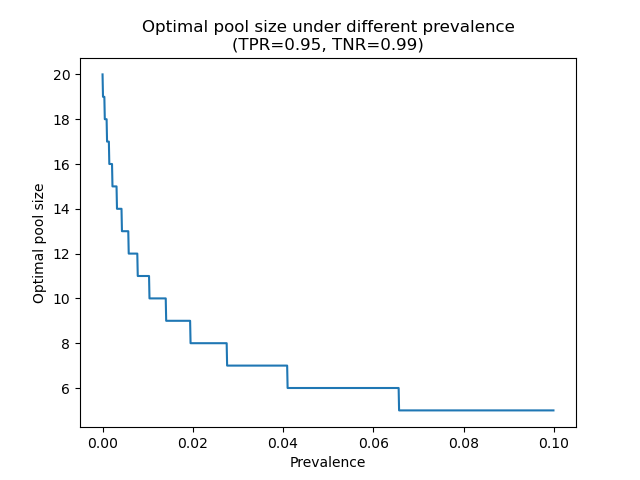
\includegraphics[width=0.65\textwidth]{model2_sample.png}
%\caption{阳性率给定,推荐混检混合样本量}
\label{model2_sample}
\end{figure}
\section{问题二的求解}
截止2022年4月底,美国累计确诊人数超过8000万人。使用美国纽约市2022年1月26日至4月26日Bronx、Brooklyn、Manhattan、Queens、Staten Island这5个区域(从前至后依次为为$\Omega_1 ,\Omega_2 ,...,\Omega_5$)的数据,对纽约市设计混检方案。

以下为5个区域的各自的人口数(从左至右依次为$n_1,n_2,...,n_5$):

\begin{table}[H]
\centering
\begin{tabular}{ccccc}
\toprule
Bronx &Brooklyn & Manhattan & Queens    & Staten Island \\
\midrule
1,418,207 & 2,559,903 & 1,628,706 & 2,253,858 &476,143     \\  
\bottomrule
\end{tabular}
\caption{纽约市各区人口数}
\end{table}
纽约市迄今没对全民做过核酸检测,所得“感染率”实际为样本平均值,公式如下:
\begin{align*}
  \rho_k(t)=  \dfrac{\mbox{当天} \Omega_{k} \mbox{阳性感染者人数}}{\mbox{当天} \Omega_{k} \mbox{参与核检总人数}}\times 100\%
\end{align*}
但我们仍可以该样本平均值反应总体平均值.

已下展示部分日期各区每日的感染率(完整数据见支撑材料):
\begin{table}[H]
\centering
\begin{tabular}{cccccc}
\toprule
End date   & Bronx & Brooklyn & Manhattan & Queens & Staten Island \\ 
\midrule
01/26/2022 & 7.26  & 7.75     & 6.74      & 10.23  & 11.71         \\
01/27/2022 & 6.67  & 7.03     & 6.15      & 9.61   & 11.19         \\
01/28/2022 & 6     & 6.53     & 5.68      & 8.79   & 10.32         \\
01/29/2022 & 5.56  & 6.06     & 5.44      & 8.18   & 9.63          \\
01/30/2022 & 5.25  & 5.62     & 5.23      & 7.66   & 9.08          \\
......     & ...... &...... &...... &...... &...... \\
\bottomrule
\end{tabular}
\caption{2022.1.26-2022.1.30每日纽约市各区阳性感染率}
\end{table}
设1月26日对应$t=1$,假设纽约市对样本的检测能力是充足的。

\subsection{利用模型一求解}
套用模型一中的情况一,得到每个地区最优的混检采样样本数$x_k$以及每日最小检测次数$\rm{min}\:w$随$t$的变化如图所示:
\begin{figure}[H]
\centering
\subfigure{
		\begin{minipage}[t]{0.4\linewidth}
			\centering          %子图居中
			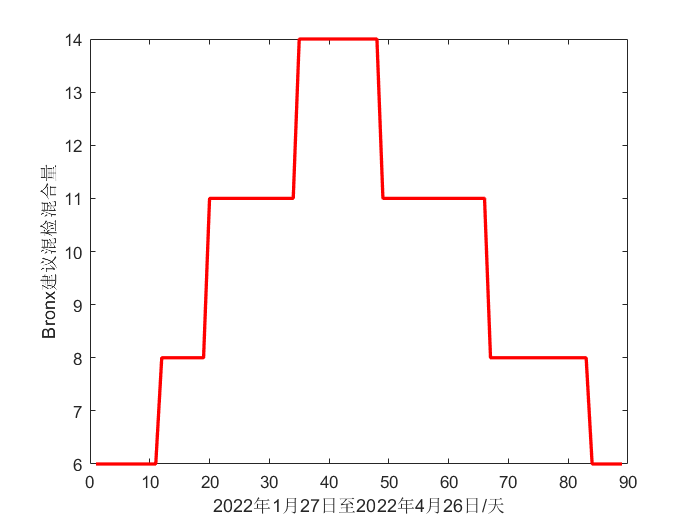
\includegraphics[scale=0.3]{Bronx建议混检混合量1.png}   %以pic.jpg的0.4倍大小输出
            \vspace{-1cm}
			\caption*{\quad \small{$x_1$随日期$t$的变化曲线图}}
		\end{minipage}
}
\subfigure{		
        \begin{minipage}[t]{0.4\linewidth}
			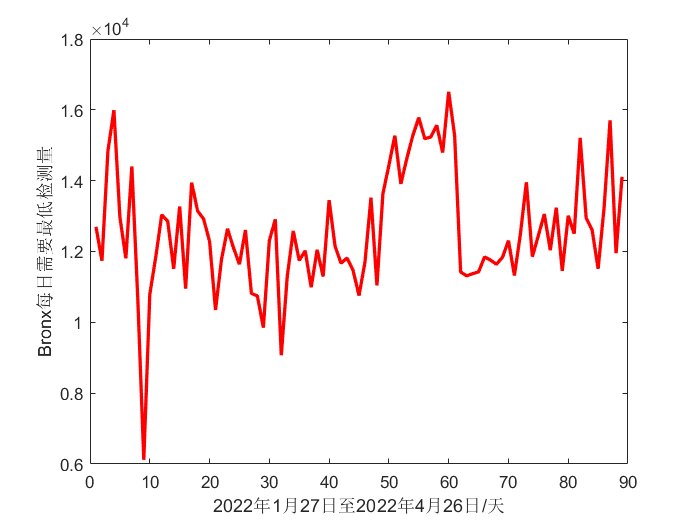
\includegraphics[scale=0.3]{Bronx每日需要最低检测量1.png}   %以pic.jpg的0.4倍大小输出
            \vspace{-1cm}
			\caption*{\quad \small{\rm{min} $w_2$随日期$t$的变化曲线图}}
		\end{minipage}
}
\caption{Bronx地区1月26日至4月26日每日的最理想混检方案} %  %大图名称
\label{fig:1}  %图片引用标记
\end{figure}

\begin{figure}[H]
\centering
\subfigure{
		\begin{minipage}[t]{0.4\linewidth}
			\centering          %子图居中
			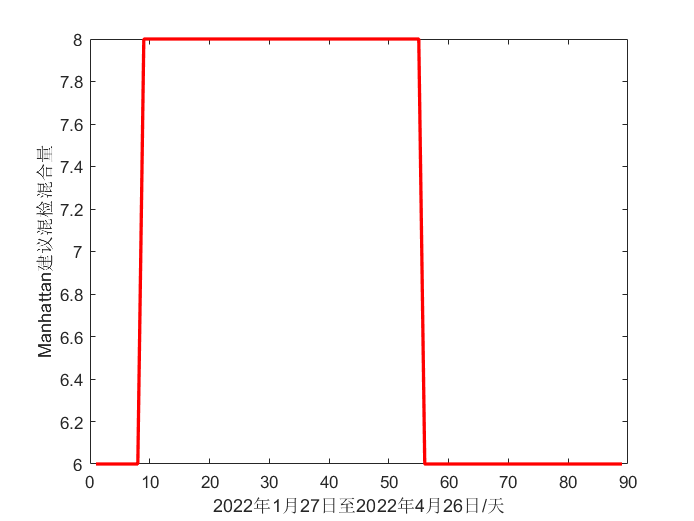
\includegraphics[scale=0.3]{布鲁克林建议混检混合量.png}   %以pic.jpg的0.4倍大小输出
            \vspace{-1cm}
			\caption*{\quad \small{$x_2$随日期$t$的变化曲线图}}
		\end{minipage}
}
\subfigure{		
        \begin{minipage}[t]{0.4\linewidth}
			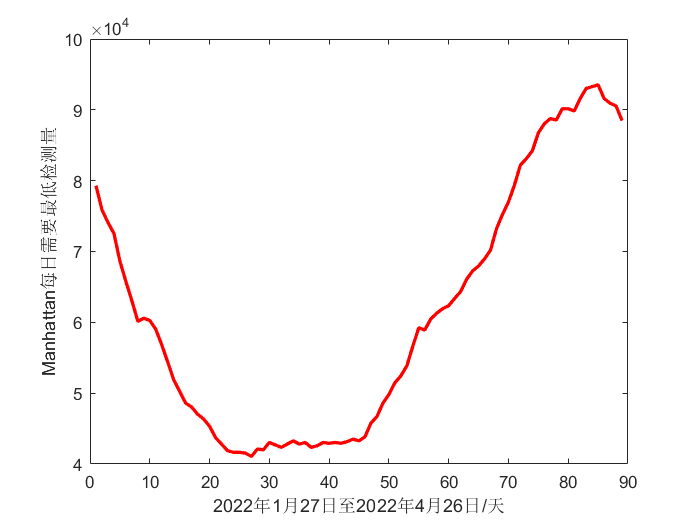
\includegraphics[scale=0.3]{布鲁克林每日需要最低检测量.png}   %以pic.jpg的0.4倍大小输出
            \vspace{-1cm}
			\caption*{\quad \small{\rm{min} $w_2$随日期$t$的变化曲线图}}
		\end{minipage}
}
\caption{Brooklyn地区1月26日至4月26日每日的最理想混检方案} %  %大图名称
\label{fig:1}  %图片引用标记
\end{figure}

\begin{figure}[H]
\centering
\subfigure{
		\begin{minipage}[t]{0.4\linewidth}
			\centering          %子图居中
			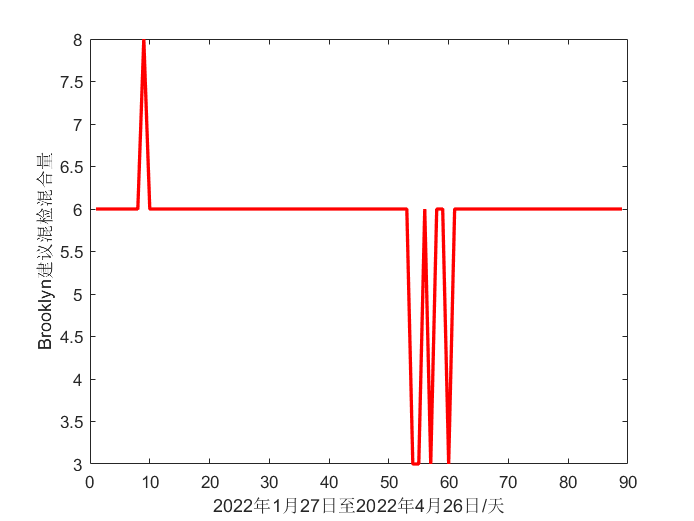
\includegraphics[scale=0.3]{Brooklyn建议混检混合量1.png}   %以pic.jpg的0.4倍大小输出
            \vspace{-1cm}
			\caption*{\quad \small{$x_3$随日期$t$的变化曲线图}}
		\end{minipage}
}
\subfigure{		
        \begin{minipage}[t]{0.4\linewidth}
			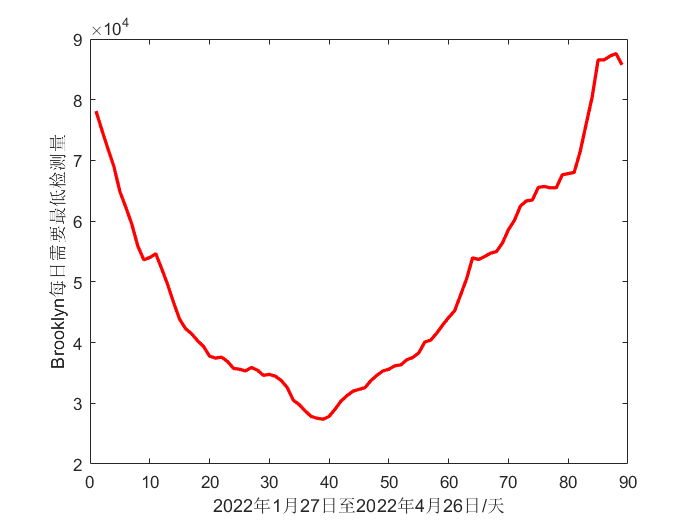
\includegraphics[scale=0.3]{Brooklyn每日需要最低检测量1.png}   %以pic.jpg的0.4倍大小输出
            \vspace{-1cm}
			\caption*{\quad \small{\rm{min} $w_3$随日期$t$的变化曲线图}}
		\end{minipage}
}
\caption{Manhattan地区1月26日至4月26日每日的最理想混检方案} %  %大图名称
\label{fig:1}  %图片引用标记
\end{figure}

\begin{figure}[H]
\centering
\subfigure{
		\begin{minipage}[t]{0.4\linewidth}
			\centering          %子图居中
			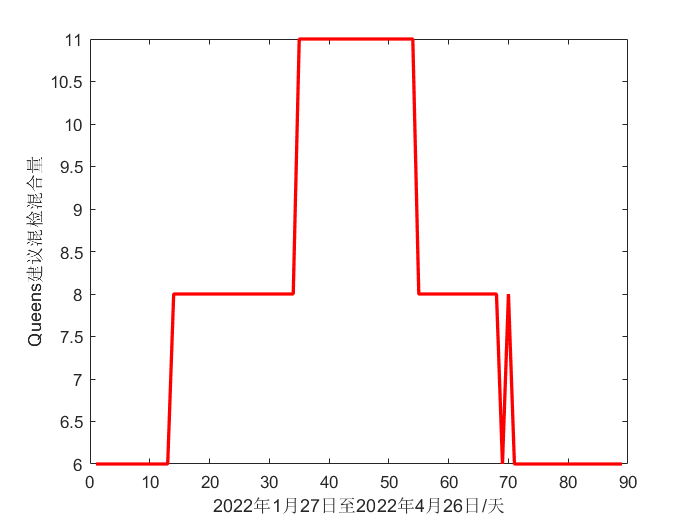
\includegraphics[scale=0.3]{Queens建议混检混合量1.png}   %以pic.jpg的0.4倍大小输出
            \vspace{-1cm}
			\caption*{\quad \small{$x_4$随日期$t$的变化曲线图}}
		\end{minipage}
}
\subfigure{		
        \begin{minipage}[t]{0.4\linewidth}
			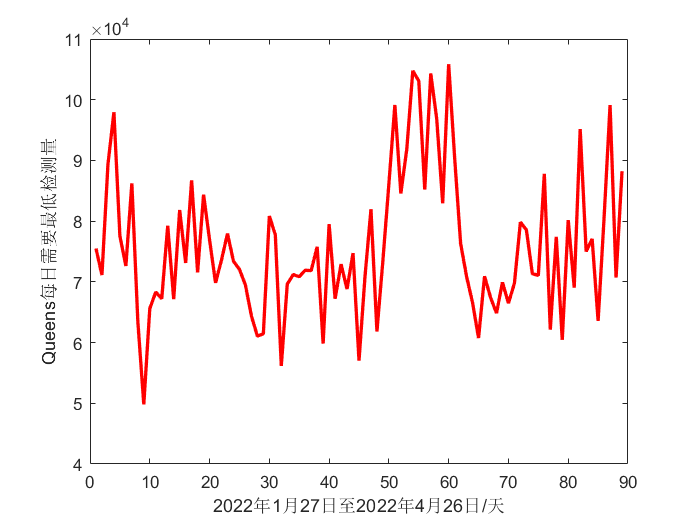
\includegraphics[scale=0.3]{Queens每日需要最低检测量1.png}   %以pic.jpg的0.4倍大小输出
            \vspace{-1cm}
			\caption*{\quad \small{\rm{min} $w_4$随日期$t$的变化曲线图}}
		\end{minipage}
}
\caption{Queens地区1月26日至4月26日每日的最理想混检方案} %  %大图名称
\label{fig:1}  %图片引用标记
\end{figure}

\begin{figure}[H]
\centering
\subfigure{
		\begin{minipage}[t]{0.4\linewidth}
			\centering          %子图居中
			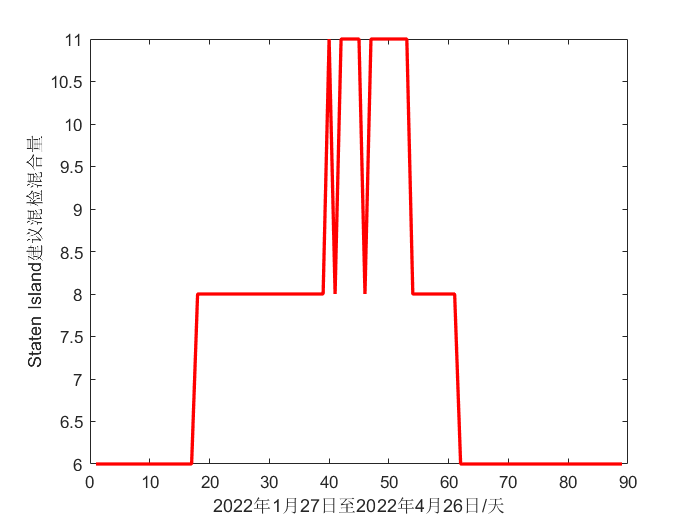
\includegraphics[scale=0.3]{Staten Island建议混检混合量1.png}   %以pic.jpg的0.4倍大小输出
            \vspace{-1cm}
			\caption*{\quad \small{$x_5$随日期$t$的变化曲线图}}
		\end{minipage}
}
\subfigure{		
        \begin{minipage}[t]{0.4\linewidth}
			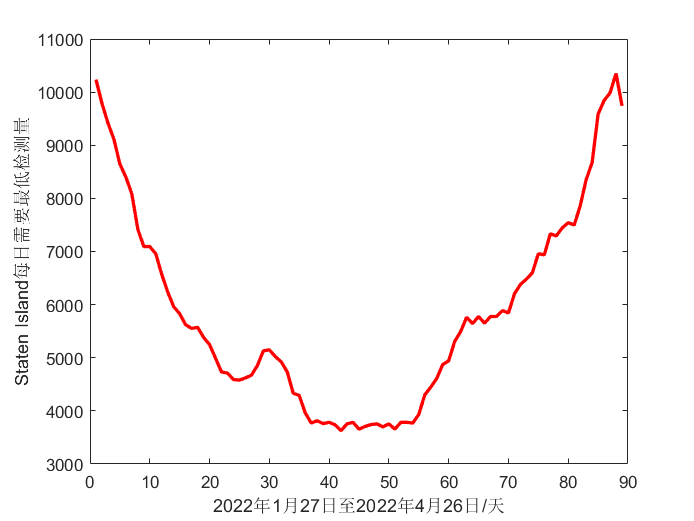
\includegraphics[scale=0.3]{Staten Island每日需要最低检测量1.png}   %以pic.jpg的0.4倍大小输出
            \vspace{-1cm}
			\caption*{\quad \small{\rm{min} $w_5$随日期$t$的变化曲线图}}
		\end{minipage}
}
\caption{Staten\ Island地区1月26日至4月26日每日的最理想混检方案} %  %大图名称
\label{fig:1}  %图片引用标记
\end{figure}

\begin{figure}[H]
\centering
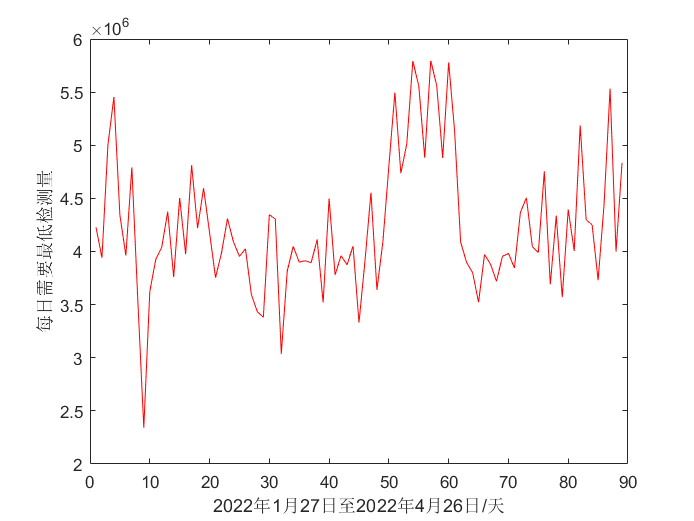
\includegraphics[width=0.5\textwidth]{fig_pro22.png}
\caption{\textbf{\rm{min} $w$随日期$t$的变化曲线图}}
\label{pro1}
\end{figure}

这些图反映了要使$w$取最小,应当根据当日不同地区新增感染率情况施行不同的混检方案,混检人数为6-11人不等,

从图中还可以看到,每日所需要的最小混检量差异较大,最少需要约$1.1 \times 10^5$次检测,而最多需约$2.4 \times 10^5$左右.

由于美国并没有采取“动态清零”的疫情防控策略,疫情的蔓延趋势在未来一定时间内仍将维持现状,从目前的的形势来看每个地区最好施行5人混检,相关部门最好可以调配至少$5 \times 10^6$次/日的单日检测力量。

\subsection{利用模型二求解}



将数据代入已经建立好的模型二,得到每个地区最优的混检采样样本数$x_k$以及每日最小检测次数$\rm {min}\:w$随$t$的变化如图所示:
\begin{figure}[H]
\centering
\subfigure{
		\begin{minipage}[t]{0.4\linewidth}
			\centering          %子图居中
			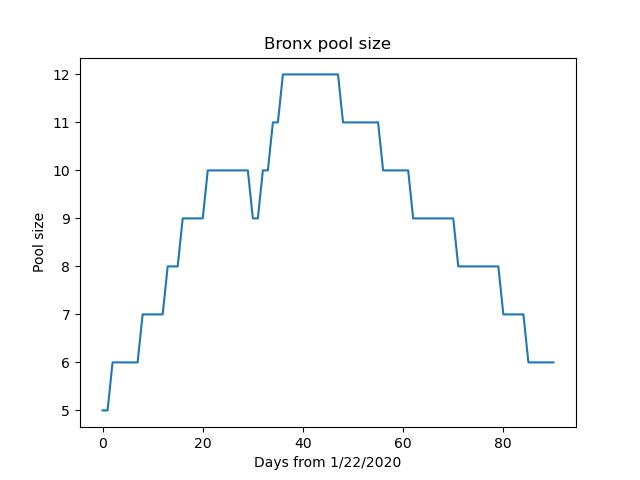
\includegraphics[scale=0.4]{nyc_Bronx_pool_size.png}  
            \vspace{-0.5cm}
			\caption*{\quad \small{$x_1$随日期$t$的变化曲线图}}
			\vspace{-0.1cm}
		\end{minipage}
}
\subfigure{		
        \begin{minipage}[t]{0.4\linewidth}
            \centering
			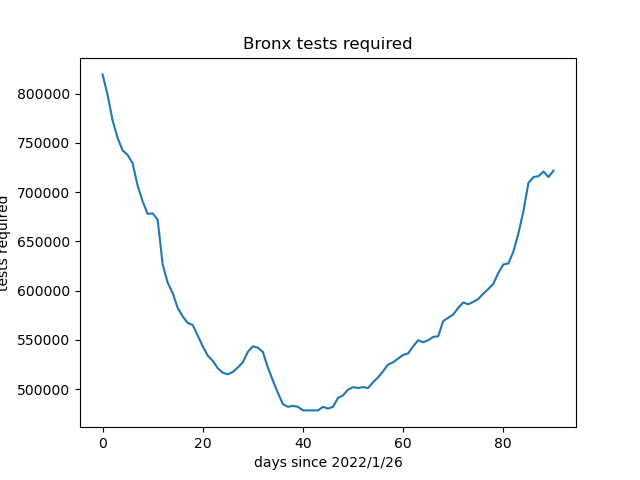
\includegraphics[scale=0.4]{nyc_Bronx_tests_to_be_conducted.png}   %以pic.jpg的0.4倍大小输出
            \vspace{-0.5cm}
			\caption*{\quad \small{\rm{min} $w_2$随日期$t$的变化曲线图}}
			\vspace{-0.1cm}
		\end{minipage}
}
\caption{Bronx地区1月26日至4月26日每日的最理想混检方案} %  %大图名称

\end{figure}

\begin{figure}[H]
\centering
\subfigure{
		\begin{minipage}[t]{0.4\linewidth}
			\centering          %子图居中
			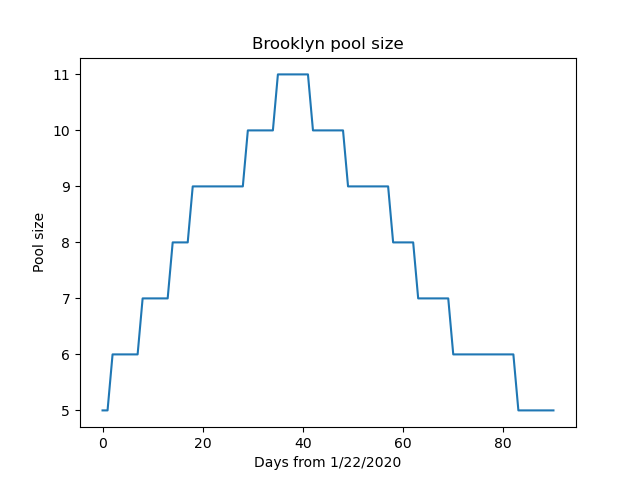
\includegraphics[scale=0.4]{nyc_Brooklyn_pool_size.png}   %以pic.jpg的0.4倍大小输出
            \vspace{-0.5cm}
			\caption*{\quad \small{$x_2$随日期$t$的变化曲线图}}
			\vspace{-0.1cm}
		\end{minipage}
}
\subfigure{		
        \begin{minipage}[t]{0.4\linewidth}
			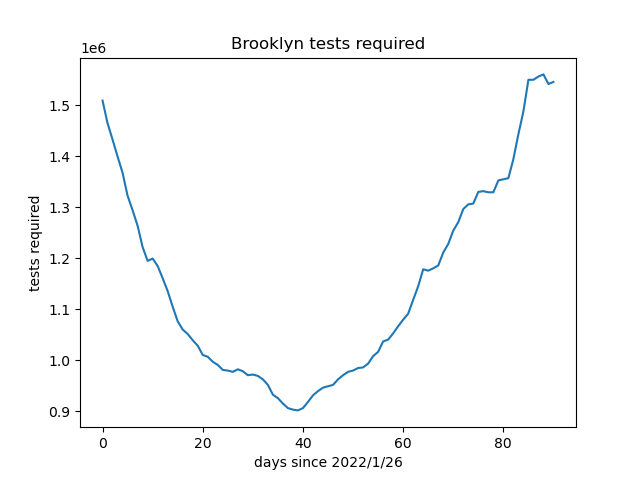
\includegraphics[scale=0.4]{nyc_Brooklyn_tests_to_be_conducted.png}   %以pic.jpg的0.4倍大小输出
            \vspace{-0.5cm}
			\caption*{\quad \small{\rm{min} $w_2$随日期$t$的变化曲线图}}
			\vspace{-0.1cm}
		\end{minipage}
}
\caption{Brooklyn地区1月26日至4月26日每日的最理想混检方案} %  %大图名称
\end{figure}

\begin{figure}[H]
\centering
\subfigure{
		\begin{minipage}[t]{0.4\linewidth}
			\centering          %子图居中
			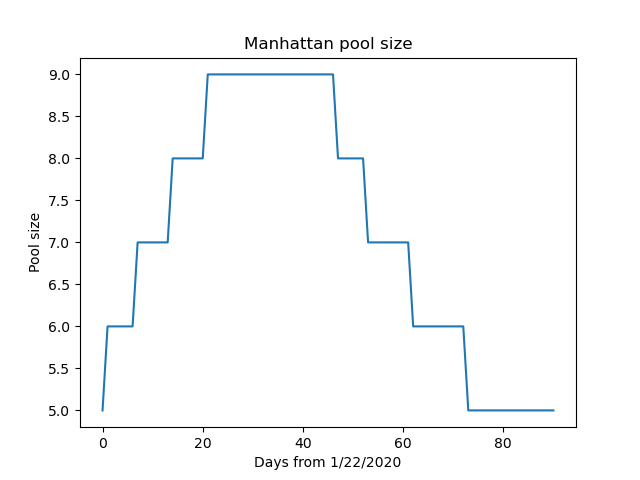
\includegraphics[scale=0.4]{nyc_Manhattan_pool_size.png}   %以pic.jpg的0.4倍大小输出
            \vspace{-0.5cm}
			\caption*{\quad \small{$x_3$随日期$t$的变化曲线图}}
			\vspace{-0.1cm}
		\end{minipage}
}
\subfigure{		
        \begin{minipage}[t]{0.4\linewidth}
			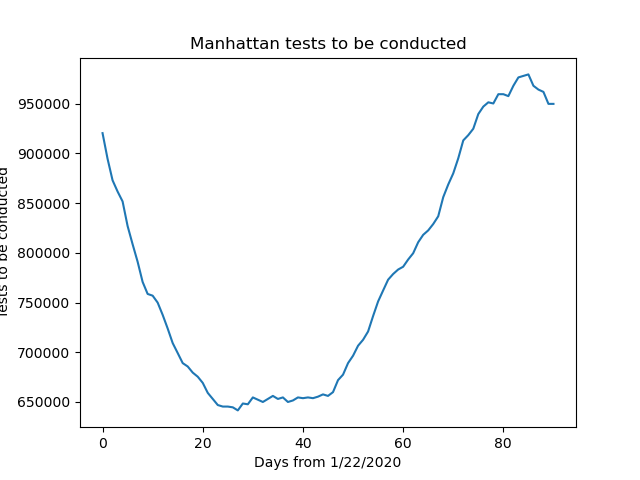
\includegraphics[scale=0.4]{nyc_Manhattan_tests_to_be_conducted.png}   %以pic.jpg的0.4倍大小输出
			\vspace{-0.5cm}
			\caption*{\quad \small{\rm{min} $w_3$随日期$t$的变化曲线图}}
			\vspace{-0.1cm}
		\end{minipage}
}
\caption{Manhattan地区1月26日至4月26日每日的最理想混检方案} %  %大图名称

\end{figure}

\begin{figure}[H]
\centering
\subfigure{
		\begin{minipage}[t]{0.4\linewidth}
			\centering          %子图居中
			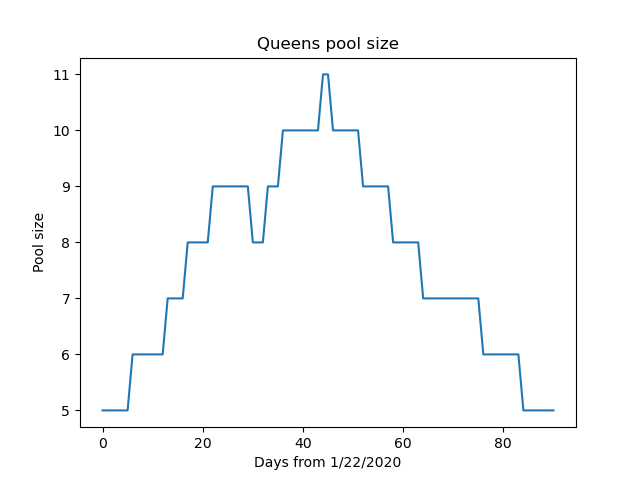
\includegraphics[scale=0.4]{nyc_Queens_pool_size.png}   %以pic.jpg的0.4倍大小输出
            \vspace{-0.5cm}
			\caption*{\quad \small{$x_4$随日期$t$的变化曲线图}}
			\vspace{-0.1cm}
		\end{minipage}
}
\subfigure{		
        \begin{minipage}[t]{0.4\linewidth}
			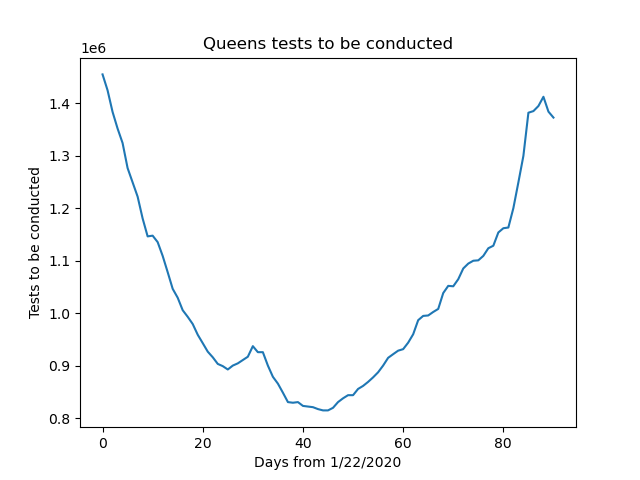
\includegraphics[scale=0.4]{nyc_Queens_tests_to_be_conducted.png}   %以pic.jpg的0.4倍大小输出
            \vspace{-0.5cm}
			\caption*{\quad \small{\rm{min} $w_4$随日期$t$的变化曲线图}}
			\vspace{-0.1cm}
		\end{minipage}
}
\caption{Queens地区1月26日至4月26日每日的最理想混检方案} %  %大图名称

\end{figure}

\begin{figure}[H]
\centering
\subfigure{
		\begin{minipage}[t]{0.4\linewidth}
			\centering          %子图居中
			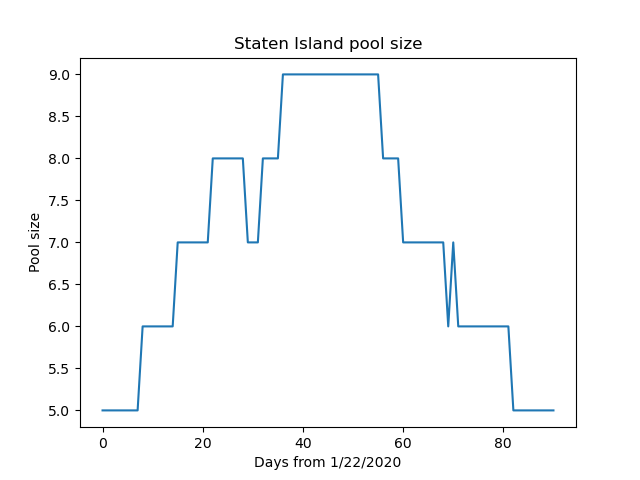
\includegraphics[scale=0.4]{nyc_Staten Island_pool_size.png}   %以pic.jpg的0.4倍大小输出
            \vspace{-0.5cm}
			\caption*{\quad \small{$x_5$随日期$t$的变化曲线图}}
			\vspace{-0.1cm}
		\end{minipage}
}
\subfigure{		
        \begin{minipage}[t]{0.4\linewidth}
			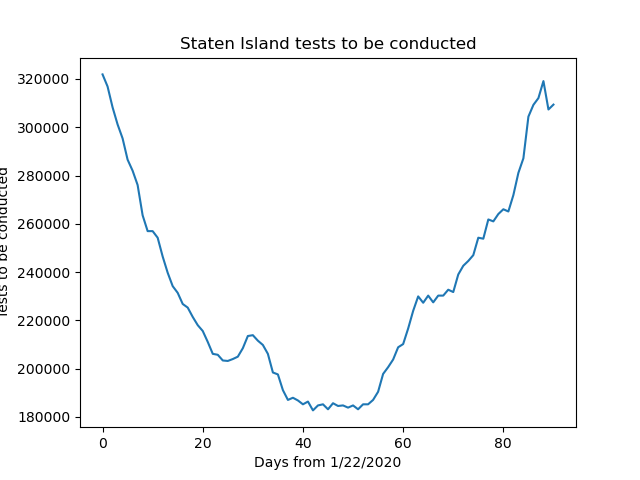
\includegraphics[scale=0.4]{nyc_Staten Island_tests_to_be_conducted.png}   %以pic.jpg的0.4倍大小输出
            \vspace{-0.5cm}
			\caption*{\quad \small{\rm{min} $w_5$随日期$t$的变化曲线图}}
			\vspace{-0.1cm}
		\end{minipage}
}
\caption{Staten\ Island地区1月26日至4月26日每日的最理想混检方案} %  %大图名称

\end{figure}

\begin{figure}[H]
\centering
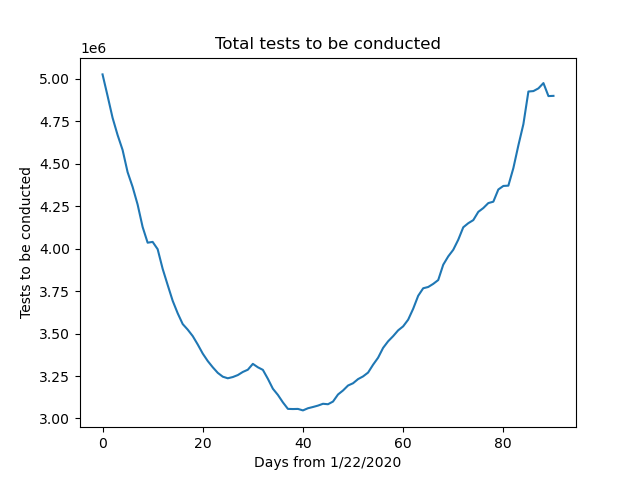
\includegraphics[width=0.5\textwidth]{nyc_total_tests_to_be_conducted.png}
\caption{\textbf{\rm{min} $w$随日期$t$的变化曲线图}}
\label{pro1}
\end{figure}

这些图反映了要使$w$取最小,应当根据当日不同地区新增感染率情况施行不同的混检方案,例如第80天除Manhattan施行5人混检,其余地区施行6人混检,

从图中还可以看到,每日所需要的最小混检量差异较大,最少需要约$3.1 \times 10^6$次检测,而最多需约$5 \times 10^6$左右.

由于美国并没有采取“动态清零”的疫情防控策略,疫情的蔓延趋势在未来一定时间内仍将维持现状,从目前的的形势来看每个地区最好施行5人混检,相关部门最好可以调配至少$5 \times 10^6$次/日的单日检测力量。

% 到此为止检查过 之前有问@5/3 1629 lty
\section{问题三模型的建立与求解}
\subsection{模型调整}
多轮检测的意义在于筛查出处于实际易感染但由于鼻咽部病毒载量(Nasopharynx viral load)过低在某轮检测中未被发现的感染者,本文后续称为U类感染者(注:潜伏期感染者是指尚未有症状的感染者,有可能已被判定为阳性,本文后续称为I类感染者)。而我们之前的模型中$\rho_k(t)$仅考虑当日可被查出的感染者,因此当日实际的感染率与$\rho_k(t)$有差异。

不妨设当日实际感染率为$\rho^*_k(t)$,则$\rho^*_k(t)$可能与$\rho_k(t)$,$\rho_k(t-1)$,...,$\rho_k(1)$相关,即:
\begin{align}
    \rho^*_k(t) = F\left(\rho_k(t),\rho_k(t-1),...,\rho_k(1) \right)
\end{align}

设判定为阳性的病毒载量为$a$,确诊最低病毒载量为$A$,不妨假设诸个体$\lambda$病毒载量一开始呈指数分布,设系数为$s_\lambda$,令设其第$t_\lambda$天低PCR指数到达$a$,第$T_\lambda$天低PCR指数到达$A$,则有:
\begin{align}
\left\{
\begin{aligned}
    & s^{t_\lambda}_{\lambda}=m; \\
    & s^{T_\lambda}_{\lambda}=M; 
\end{aligned}
    \right.
    \Rightarrow & \dfrac{T_\lambda}{t_\lambda}=\dfrac{\ln A}{\ln a}=c
\end{align}
通俗来说即:确诊时间与到达阳性时间之比为定值,与个体无关。

令$P(t-1<\xi \leqslant t)$表示潜伏期为$t$天的概率,假设$\xi$服从分布的密度函数为$f(t)$给定(可由统计得到),令设$P(t-1< \eta \leqslant t)$表示确定为阳性需$t$天的概率,故$\eta$服从分布的密度函数为$g(t)=f(ct)$.

第$t-1$天未被判定为阳性的感染者的比例为$\rho^*_k(t-1)-\rho_k(t-1)$,得递推式:
\begin{align}
\left\{
\begin{aligned}
    & \rho^*_k(1),\rho_k(1)\quad {\rm given.}\\
    & \rho^*_k(2) =\rho_k(2) +\int^1_0 f(cx)dx\cdot \left(\rho^*_k(1)-\rho_k(1) \right)   \\
    & ...  \\
    & \rho^*_k(t) =\rho_k(t) + \sum^{t-1}_{i=1} \int^i_{i-1} f(cx)dx \cdot \left(\rho^*_k(t-i)-\rho_k(t-i) \right) 
\end{aligned}
 \right.  
\end{align}

从而将模型一、模型二中的$\rho_k(t),\rho_k(t-1)$替换成$\rho^*_k(t),\rho^*_k(t-1)$即可.

\subsection{模型求解}
由于对模型一、模型二的调整仅仅是将参数$\rho_k(t)$改为$\rho^*_k(t)$,因此解法不用更改。

根据Covid-19 Alpha病毒的潜伏期分布图\cite{wuhan},又Omicron患者自暴露感染源至检测呈阳性的平均周期为3.5天,推测$\eta$近似服从$ \chi^2  \left(3.5\right)$,密度函数为:
\begin{align}
    g(t)= \dfrac{1}{2^1.75 \cdot \Gamma \left(1.75 \right)}t^{0.75}\exp \left(\dfrac{t}{2} \right) \quad t\geqslant0 
\end{align}

我们首先将纽约五大地区1月26日至4月26日的感染率数据代入式29、30,以求$\rho^*_k(t)$,约定符号与问题二相同,得到:

\begin{table}[H]
\centering
\begin{tabular}{ccccccc}
\toprule
时间 & Bronx实 & Bronx测 & Brooklyn实 & Brooklyn测 & Manhattan & Manhattan \\
     & 际感染率& 得感染率& 际感染率& 得感染率际  &实际感染率   &测得感染率\\
     & $\rho^*_1(t)$ & $\rho_1(t)$& $\rho^*_2(t)$& $\rho_2(t)$  &$\rho^*_3(t)$   &$\rho_3(t)$\\
\midrule
01/26/2022 & 7.99       & 7.26       & 7.99          & 7.75          & 7.41           & 6.74           \\
01/27/2022 & 6.77       & 6.67       & 6.77          & 7.03          & 6.24           & 6.15           \\
01/28/2022 & 6.16       & 6.00       & 6.16          & 6.53          & 5.83           & 5.68           \\
01/29/2022 & 5.74       & 5.56       & 5.74          & 6.06          & 5.60           & 5.44           \\
01/30/2022 & 5.43       & 5.25       & 5.43          & 5.62          & 5.40           & 5.23           \\
01/31/2022 & 5.32       & 5.14       & 5.32          & 5.02          & 4.89           & 4.72           \\
02/01/2022 & 5.12       & 4.94       & 5.12          & 4.65          & 4.52           & 4.35           \\
02/02/2022 & 4.59       & 4.41       & 4.59          & 4.26          & 4.18           & 4.01           \\
02/03/2022 & 4.23       & 4.05       & 4.23          & 3.77          & 3.82           & 3.65           \\
02/04/2022 & 3.97       & 3.79       & 3.97          & 3.47          & 3.61           & 3.44           \\
......     & ......     & ......     & ......        & ......        & ......         & ......        \\
\bottomrule
\end{tabular}
\caption{2022.1.26-2022.1.30每日纽约市各区测得与实际阳性感染率}
\end{table}

以Manhattan($\Omega_3$)的数据为例,如图为与$\rho_3(t)$与$\rho^*_3(t)$的对比图:
\begin{figure}[H]
\centering
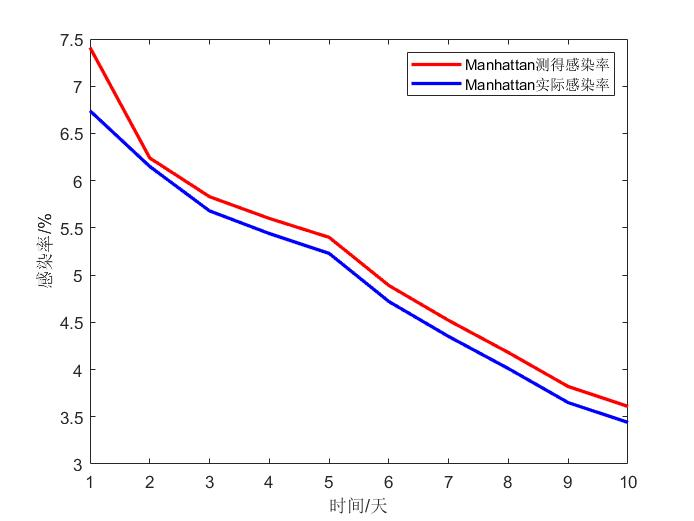
\includegraphics[width=0.5\textwidth]{rho_Manhattan.jpg}% TODO: replace your plot here, delete me after completion
\caption{\textbf{Manhattan$\rho_3(t)$与$\rho^*_3(t)$的对比图}}
\label{pro1}
\end{figure}

随着$t$的增大$\rho^*_k(t)$与$\rho_k(t)$差异越来越小,趋势也也来越相同,因此可以推断随着$t$的增大,结论也将趋于问题二得出的结论。

不妨以Manhattan($\Omega_3$)的数据为例分析,同样默认检测资源充足:

以下为模型一的结果,红线为我们之前得到的结果,蓝线为我们将$\rho_3(t)$改为$\rho^*_3(t)$的结果。
\begin{figure}[H]
\centering
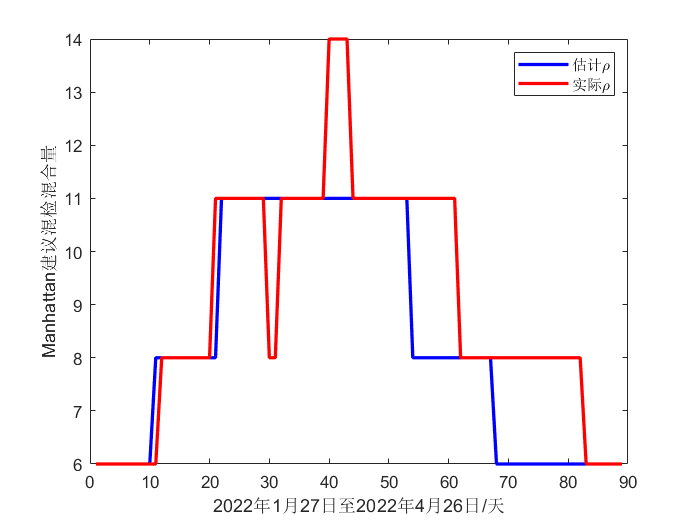
\includegraphics[width=0.5\textwidth]{Manhattan对比混检样本数量1.png}
\caption{\textbf{$x_3$随日期$t$的变化曲线图}}
\label{pro1}
\end{figure}

以下为模型二的结果,红线为我们之前得到的结果,蓝线为我们将$\rho_3(t)$改为$\rho^*_3(t)$的结果。
\begin{figure}[H]
\centering
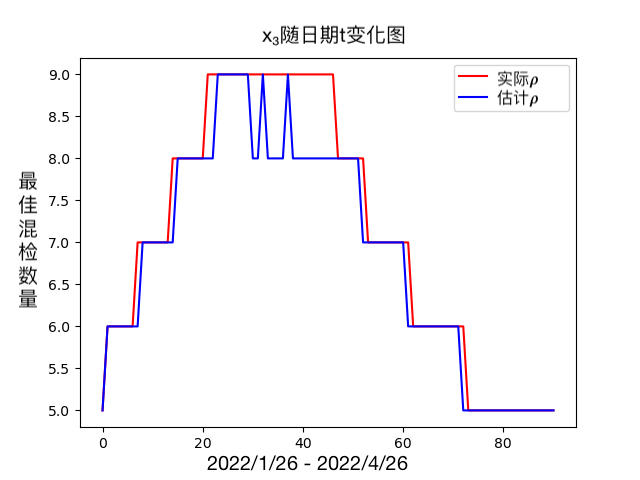
\includegraphics[width=0.5\textwidth]{q3.png}
\caption{\textbf{$x_3$随日期$t$的变化曲线图}}
\label{pro1}
\end{figure}

\section{模型分析} 
\subsection{灵敏度分析}
灵敏度分析是研究与分析一个模型的状态或输出变化对系统参数或周围条件变化的敏感程度的方法。

在建立的模型中,共有三个超参数:阳性率、真阳率、真阴率。对其分别增加1后,对模型均方误差的变化,记录下表\ref{模型灵敏度分析}。

\begin{table}[H]
\caption{模型灵敏度分析}
\label{模型灵敏度分析}
\centering
\begin{tabular}{llllll}
\toprule
参数 & 数值   & 增加量 & 变化后数值 & 变化后混检人数 & 混检人数的变化\\
\midrule
阳性率$\rho$ & 0.05 & 10$\%$ & 0.06  & 7   & 16.67$\%$  \\
真阳率TPR  & 0.95 & 3\%  & 0.98  & 6   & 0\%   \\
真阴率TNR  & 0.99 & 1\%  & 0.995  & 6   & 0\%  \\
\bottomrule
\end{tabular}
\end{table}

如上表\ref{模型灵敏度分析},超参数的微小改变仅带来因变量的微小扰动,说明模型灵敏度较好。同时超参数的增加或减小均会降低模型精确度,说明超参数已经达到最佳。


\section{模型评价} % TODO
\subsection{模型优缺点}
\subsubsection{模型优点}
\begin{itemize}
    \item 讨论了新冠检测能力充足、有限及严重不足时的最佳混检策略,能够适应各种现实情况。
    
    \item 模型二在算法的时间复杂度为$O(N)$,即线性时间复杂度,运行速度快,可以在短时间内计算得出结果。
    
    \item 模型二考虑了真假阳性的情况,对概率的真实值进一步优化.
    \item 结合多轮混检的意义基于统计分布和已有数据进一步优化模型参数,从而得到更合理的结论.
\end{itemize}

\subsubsection{模型缺点}
\begin{itemize}
    \item 模型一情况2、3求解效率低,对大批量的数据处理耗时过长。
    
    \item 模型仅考虑了感染率,忽略了治愈率和潜在感染风险
    
    \item 模型的参数都是基于已记录的数据和已发生的事件给出结论,不能根据数据预测未来的数据并设为新参数,因此结论只适用于过去以及短期未来,不适用于长期未来。
\end{itemize}

\subsection{模型的改进与推广}
\begin{itemize}
    \item 可反向利用模型推测当然的感染率数据是否合理,比如已知地区$\Omega_k$的人口。施行多少人一混检的策略,复检资源分配情况,反推出当日的感染率。
    
    \item 可参照SEIR等传染病模型,并将疫情管控措施对传染的影响加入考量,进一步细化对感染者分布的估计,从而得出更为准确之结果。
    
    \item 模型鲁棒性强,其他任何流行病传染问题均都可以运用我们的模型来计算最佳混检样本数量
\end{itemize}

\newpage

\begin{thebibliography}{100}
\bibitem{columbia}Columbia University. COVID-19 testing program for Spring 2022. Retrieved May 3, 2022, from https://covid19.columbia.edu/content/covid-19-testing-program-spring-2022
\bibitem{max_maps}
Yelin, Idan, et al. "Evaluation of COVID-19 RT-qPCR test in multi sample pools." Clinical Infectious Diseases 71.16 (2020): 2073-2078.
\bibitem{bib1}Christopher D Pilcher, Daniel Westreich, Michael G Hudgens, Group Testing for Severe Acute Respiratory Syndrome– Coronavirus 2 to Enable Rapid Scale-up of Testing and Real-Time Surveillance of Incidence, The Journal of Infectious Diseases, Volume 222, Issue 6, 15 September 2020, Pages 903–909
\bibitem{bib20}郭志军.分支定界算法的MATLAB实现[J].江西教育学院学报,2007(06):4-7.
\bibitem{hunan}潘静静, 王莹莹, 王文华, et al. 一起由奥密克戎变异株BA.2.2引起的河南省新冠肺炎本土疫情流行病学特征分析[J]. 中国公共卫生, 2022, 38(5):1-5.
\bibitem{wuhan}Hahakity. 新冠肺炎潜伏期分布统计. Retrieved May 4, 2022, from https://zhuanlan.zhihu.com/p/104670786
\bibitem{bib2}Berger, T., J. W. Mandell, and P. Subrahmanya. 2000. Maximally efficient two-stage screening. Biometrics 56:833–840.
\bibitem{bib3}Westreich, Daniel J., et al. "Optimizing screening for acute human immunodeficiency virus infection with pooled nucleic acid amplification tests." Journal of Clinical Microbiology 46.5 (2008): 1785-1792.
\bibitem{bib4}董宏杰, et al. "新型冠状病毒混合样品检测研究." 山东大学学报 (医学版) 59.4 (2021): 1-5.
\bibitem{bib5}Kline, Richard L., et al. "Evaluation of human immunodeficiency virus seroprevalence in population surveys using pooled sera." Journal of clinical microbiology 27.7 (1989): 1449-1452.

\end{thebibliography}

\newpage

\begin{appendices}
\section{数据}
\subsection{附录指南}
\begin{table}[H]
\centering
\begin{tabular}{ll}
\toprule
编号    & 内容        \\
\midrule
1.2   & 问题二、三原始数据 \\
2.1.1 & 问题一模型一代码  \\
2.1.2 & 问题一模型二代码  \\
2.2.1 & 问题二模型一代码  \\
2.2.2 & 问题二模型二代码  \\
2.3.1 & 问题三代码    \\
\bottomrule
\end{tabular}
\caption{附录指南}
\end{table}

\subsection{问题二、三原始数据}
\begin{center}
\begin{longtable}{c|ccccc}
\toprule
End date   & Bronx & Brooklyn & Manhattan & Queens & Staten Island \\
\midrule
01/26/2022 & 7.26  & 7.75     & 6.74      & 10.23  & 11.71         \\
01/27/2022 & 6.67  & 7.03     & 6.15      & 9.61   & 11.19         \\
01/28/2022 & 6     & 6.53     & 5.68      & 8.79   & 10.32         \\
01/29/2022 & 5.56  & 6.06     & 5.44      & 8.18   & 9.63          \\
01/30/2022 & 5.25  & 5.62     & 5.23      & 7.66   & 9.08          \\
01/31/2022 & 5.14  & 5.02     & 4.72      & 6.79   & 8.27          \\
02/01/2022 & 4.94  & 4.65     & 4.35      & 6.33   & 7.86          \\
02/02/2022 & 4.41  & 4.26     & 4.01      & 5.9    & 7.34          \\
02/03/2022 & 4.05  & 3.77     & 3.65      & 5.26   & 6.3           \\
02/04/2022 & 3.79  & 3.47     & 3.44      & 4.75   & 5.81          \\
02/05/2022 & 3.8   & 3.52     & 3.41      & 4.77   & 5.81          \\
02/06/2022 & 3.67  & 3.36     & 3.29      & 4.59   & 5.61          \\
02/07/2022 & 2.78  & 3.1      & 3.08      & 4.21   & 5.05          \\
02/08/2022 & 2.46  & 2.83     & 2.85      & 3.8    & 4.58          \\
02/09/2022 & 2.28  & 2.53     & 2.62      & 3.4    & 4.2           \\
02/10/2022 & 2.03  & 2.26     & 2.47      & 3.19   & 4.02          \\
02/11/2022 & 1.89  & 2.11     & 2.32      & 2.9    & 3.74          \\
02/12/2022 & 1.79  & 2.03     & 2.27      & 2.75   & 3.65          \\
02/13/2022 & 1.76  & 1.92     & 2.18      & 2.6    & 3.42          \\
02/14/2022 & 1.6   & 1.83     & 2.12      & 2.38   & 3.22          \\
02/15/2022 & 1.44  & 1.68     & 2.03      & 2.21   & 3.08          \\
02/16/2022 & 1.31  & 1.65     & 1.89      & 2.04   & 2.82          \\
02/17/2022 & 1.24  & 1.57     & 1.81      & 1.93   & 2.56          \\
02/18/2022 & 1.14  & 1.52     & 1.73      & 1.81   & 2.54          \\
02/19/2022 & 1.08  & 1.44     & 1.71      & 1.77   & 2.42          \\
02/20/2022 & 1.06  & 1.43     & 1.71      & 1.71   & 2.41          \\
02/21/2022 & 1.09  & 1.41     & 1.7       & 1.78   & 2.45          \\
02/22/2022 & 1.15  & 1.45     & 1.66      & 1.82   & 2.5           \\
02/23/2022 & 1.22  & 1.42     & 1.75      & 1.88   & 2.68          \\
02/24/2022 & 1.36  & 1.36     & 1.74      & 1.94   & 2.96          \\
02/25/2022 & 1.44  & 1.37     & 1.83      & 2.15   & 2.98          \\
02/26/2022 & 1.42  & 1.35     & 1.8       & 2.03   & 2.85          \\
02/27/2022 & 1.36  & 1.3      & 1.77      & 2.03   & 2.75          \\
02/28/2022 & 1.15  & 1.22     & 1.81      & 1.78   & 2.56          \\
03/01/2022 & 0.98  & 1.08     & 1.85      & 1.58   & 2.17          \\
03/02/2022 & 0.83  & 1.03     & 1.81      & 1.46   & 2.13          \\
03/03/2022 & 0.7   & 0.96     & 1.83      & 1.31   & 1.82          \\
03/04/2022 & 0.67  & 0.9      & 1.77      & 1.16   & 1.64          \\
03/05/2022 & 0.68  & 0.88     & 1.79      & 1.15   & 1.68          \\
03/06/2022 & 0.67  & 0.87     & 1.83      & 1.16   & 1.63          \\
03/07/2022 & 0.63  & 0.9      & 1.82      & 1.1    & 1.56          \\
03/08/2022 & 0.63  & 0.98     & 1.83      & 1.09   & 1.61          \\
03/09/2022 & 0.63  & 1.07     & 1.82      & 1.08   & 1.45          \\
03/10/2022 & 0.63  & 1.13     & 1.84      & 1.05   & 1.54          \\
03/11/2022 & 0.67  & 1.18     & 1.87      & 1.03   & 1.56          \\
03/12/2022 & 0.65  & 1.2      & 1.85      & 1.03   & 1.47          \\
03/13/2022 & 0.67  & 1.22     & 1.9       & 1.07   & 1.58          \\
03/14/2022 & 0.77  & 1.3      & 2.07      & 1.16   & 1.53          \\
03/15/2022 & 0.8   & 1.36     & 2.15      & 1.22   & 1.54          \\
03/16/2022 & 0.87  & 1.41     & 2.32      & 1.27   & 1.5           \\
03/17/2022 & 0.9   & 1.43     & 2.43      & 1.27   & 1.54          \\
03/18/2022 & 0.89  & 1.47     & 2.58      & 1.37   & 1.47          \\
03/19/2022 & 0.9   & 1.48     & 2.67      & 1.42   & 1.56          \\
03/20/2022 & 0.89  & 1.54     & 2.8       & 1.49   & 1.56          \\
03/21/2022 & 0.96  & 1.66     & 3.06      & 1.57   & 1.64          \\
03/22/2022 & 1.02  & 1.73     & 3.31      & 1.66   & 1.79          \\
03/23/2022 & 1.1   & 1.9      & 3.5       & 1.78   & 2.14          \\
03/24/2022 & 1.19  & 1.93     & 3.69      & 1.92   & 2.28          \\
03/25/2022 & 1.22  & 2.04     & 3.79      & 1.99   & 2.44          \\
03/26/2022 & 1.27  & 2.17     & 3.87      & 2.06   & 2.7           \\
03/27/2022 & 1.32  & 2.29     & 3.92      & 2.09   & 2.77          \\
03/28/2022 & 1.34  & 2.4      & 4.05      & 2.22   & 3.14          \\
03/29/2022 & 1.44  & 2.66     & 4.17      & 2.39   & 3.57          \\
03/30/2022 & 1.53  & 2.93     & 4.39      & 2.68   & 3.93          \\
03/31/2022 & 1.5   & 3.29     & 4.54      & 2.77   & 3.77          \\
04/01/2022 & 1.53  & 3.26     & 4.63      & 2.78   & 3.95          \\
04/02/2022 & 1.58  & 3.31     & 4.76      & 2.86   & 3.78          \\
04/03/2022 & 1.59  & 3.37     & 4.92      & 2.93   & 3.95          \\
04/04/2022 & 1.82  & 3.65     & 5.32      & 3.3    & 3.95          \\
04/05/2022 & 1.87  & 3.84     & 5.59      & 3.47   & 4.1           \\
04/06/2022 & 1.92  & 4.14     & 5.83      & 3.46   & 4.04          \\
04/07/2022 & 2.03  & 4.35     & 6.16      & 3.63   & 4.53          \\
04/08/2022 & 2.12  & 4.68     & 6.56      & 3.89   & 4.78          \\
04/09/2022 & 2.09  & 4.8      & 6.69      & 4.01   & 4.92          \\
04/10/2022 & 2.13  & 4.82     & 6.85      & 4.08   & 5.09          \\
04/11/2022 & 2.18  & 5.12     & 7.22      & 4.09   & 5.61          \\
04/12/2022 & 2.27  & 5.14     & 7.41      & 4.21   & 5.58          \\
04/13/2022 & 2.35  & 5.11     & 7.52      & 4.42   & 6.17          \\
04/14/2022 & 2.44  & 5.11     & 7.49      & 4.49   & 6.11          \\
04/15/2022 & 2.63  & 5.42     & 7.73      & 4.86   & 6.34          \\
04/16/2022 & 2.78  & 5.45     & 7.73      & 4.98   & 6.49          \\
04/17/2022 & 2.8   & 5.48     & 7.68      & 5      & 6.42          \\
04/18/2022 & 3.03  & 5.99     & 7.95      & 5.56   & 6.98          \\
04/19/2022 & 3.39  & 6.69     & 8.17      & 6.33   & 7.78          \\
04/20/2022 & 3.84  & 7.4      & 8.21      & 7.21   & 8.32          \\
04/21/2022 & 4.47  & 8.43     & 8.25      & 8.76   & 9.94          \\
04/22/2022 & 4.61  & 8.43     & 7.95      & 8.82   & 10.42         \\
04/23/2022 & 4.63  & 8.54     & 7.85      & 9.01   & 10.7          \\
04/24/2022 & 4.74  & 8.61     & 7.79      & 9.36   & 11.42         \\
04/25/2022 & 4.61  & 8.29     & 7.48      & 8.8    & 10.23         \\
04/26/2022 & 4.76  & 8.36     & 7.48      & 8.58   & 10.43 
\\
\bottomrule
\end{longtable}
\end{center}

\section{代码}
\subsection{问题一}
\subsubsection{模型一代码}
\begin{lstlisting}[language = matlab]
all_data = xlsread('positive.csv');
nk = xlsread('pop.xlsx');
% % import all data

w0 = 100;
% The maximun detection numbers, which is very huge
N = 3;
% numbers of blocks we use
num = 2;
% length odf time we use; pay attention that N is larger than 2
rho = all_data(7:6 + N,1:num)./100;
% the rho we need
rho([1,2],:)=rho([2,1],:);% A magical operation, we need to delete later
nk = nk(1:N);
% the population we need

t = 2;
% today is 2

rhox = 0.001:0.001:0.02;
xx = [];

w0 = 100000;
% The maximun detection numbers, which is very huge
N = 3;
% numbers of blocks we use
num = 2;

t = 2;

x_min = 1;
% x_min is what we want
w = 0;
x = 10;
% When we fix x, we can get w0
for i = 1:N
    w = w + round(nk(i) / x + 0.5) + nk(i) * max(0,1 - (1 - rho^ x));
end
w_min = w;

% We use Newton method here
key = 1;

x = [0,32];
while key == 1
    x1 = round(0.382 * (x(2) - x(1)) + x(1));
    x2 = round(0.618 * (x(2) - x(1)) + x(1));
    w1 = 0;
    w2 = 0;
    for i = 1:N
        w1 = w1 + round(nk(i) / x1 + 0.5) + nk(i) * max(0,1 - (1 - rho)^ x1);
        w2 = w2 + round(nk(i) / x2 + 0.5) + nk(i) * max(0,1 - (1 - rho)^ x2);
    end
    if w1 >= w2
        x = [x1,x(2)];
    else
        x = [x(1),x2];
    end
    if abs(x(2) - x(1)) <= 1
        x1 = round(0.382 * (x(2) - x(1)) + x(1));
        x2 = round(0.618 * (x(2) - x(1)) + x(1));
        w1 = 0;
        w2 = 0;
        for i = 1:N
            w1 = w1 + round(nk(i) / x1 + 0.5) + nk(i) * max(0,1 - (1 - rho)^ x1);
            w2 = w2 + round(nk(i) / x2 + 0.5) + nk(i) * max(0,1 - (1 - rho)^ x2);
        end
        if w1 > w2
            x_min = x(2);
            w_min = w2;
        else
            x_min = x(1);
            w_min = w1;
        end
        key = 0;
    end
end

xx(j) = x_min ;

end
plot(rhox,xx,'r','linewidth',2)
xlabel('阳性率/%')
ylabel('混检混合样本量/人')

\end{lstlisting}

\subsubsection{模型二代码}
求解函数库 optimal.py:
\begin{lstlisting}[language = python]
"""
Obtain optimal pooling strategy.

By scoring and comparing every possible COVID-19 test pooling strategy, find
the best strategy.

Typical using example:
optimal_x,optimal_score=(opts(rho,tpr,tnr))
"""

from cmath import log

def s(x,rho,tpr,tnr,xlb,xrb):
    """
    Scoring the pooling strategy .
    
    Return the expectation of tests to be conducted per person, the smaller the
    better.

    Args:
        x: Pool size
        rho: Prevalence in given sample
        tpr: True positive rate (aka. sensitivity, P{TP}/(P{TP}+P{FN})) of the
             test
        tnr: True negative rate (aka. specificity, P{TN}/(P{TN}+P{FP})) of the
             test
        xlb: Lower bound of the pool size, 2 by default
        xlb: Upper bound of the pool size, 32 by default
    
    Returns:
        An int evaluating given case. Return None if args exceeds boundaries.
    """
    # Check boundaries
    if x<xlb or x>xrb or int(x)!=x:
        return None
    if rho>1 or rho<0:
        return None
    if tpr>1 or tpr<0:
        return None
    if tnr>1 or tnr<0:
        return None
    # Calculate tpr after the dilution
    tpr_diluted=tpr*(1-log(x,10).real/7)
    # Calculate E[S]
    s_P=x+1
    s_N=1
    p_TP=(1-(1-rho)**x)*tpr_diluted
    p_FP=(1-rho)**x*(1-tpr_diluted)
    p_TN=(1-rho)**x*tnr
    p_FN=(1-(1-rho)**x)*(1-tnr)
    return (s_P*(p_TP+p_FP)+s_N*(p_TN+p_FN))/x

def opts(rho,tpr,tnr,xlb=2,xrb=32):
    """
    Find the best pool size.

    Find the best pool size of the given case by iterating the evaluation with
    size ranging from min to max.

    Args:
        rho: Prevalence in given sample
        tpr: True positive rate (aka. sensitivity, P{TP}/(P{TP}+P{FN})) of the
             test
        tnr: True negative rate (aka. specificity, P{TN}/(P{TN}+P{FP})) of the
             test
        xlb: Lower bound of the pool size, 2 by default
        xlb: Upper bound of the pool size, 32 by default

    Returns:
        A tuple of int consisting optimal pool size and its score.
    """
    opt_s=999
    opt_x=-1
    for i in range(xlb,xrb+1):
        new_s= s(i,rho,tpr,tnr,xlb,xrb)
        if(new_s<opt_s):
            opt_s=new_s
            opt_x=i
    return opt_x,opt_s

\end{lstlisting}
示例 q1$\_$sample.py:
\begin{lstlisting}[language=python]
"""
Samples for question 1.

Samples for question 1 including a terminal print and a chart revealing the
corresponding optimal pool size given by the model under different prevalence.
"""

from optimal import opts
import numpy as np
import matplotlib.pyplot as plt

# Sample of the case which rho=.05, tpr=.95, tnr=.99
rho,tpr,tnr=0.05,0.95,0.99
opt_x,opt_s=(opts(rho,tpr,tnr))
print("示例 ("+"rho="+str(rho)+", TPR="+str(tpr)+", TNR="+str(tnr)+"):")
print("\t最佳混检池大小 = "+str(opt_x))
print("\t相应评分 = "+str(opt_s))

# Plot optimal pool size for different prevalence
rho=np.arange(0,0.1,0.0001)
tpr,tnr=0.95,0.99
x=[]
y=[]
for i in rho:
    x.append(opts(i,tpr,tnr)[0])
    y.append(opts(i,tpr,tnr)[1])
plt.plot(rho,x)
plt.title("Optimal pool size under different prevalence\n(TPR="+str(tpr)+", TNR="+str(tnr)+")")
plt.xlabel("Prevalence")
plt.ylabel("Optimal pool size")
plt.savefig("model2_sample.png")
\end{lstlisting}
\subsection{问题二代码}
\subsubsection{模型一代码}
\begin{lstlisting}[language = matlab]
rho = [0.01,0.02];
nk = [4000,3000]
w_0 = 2000;

xx = 1:1:32
zz = [];
for j = 1:32
x = xx(j);

f_x = (1 - (1 - rho).^x);

rho_star = rho;
c = - rho_star .* x .* f_x;
a = (f_x .*x + ones(size(f_x)));
b = w_0;
[uk,f]=ILp(c,a,b,[],[],zeros(1,length(f_x)),w_0.*ones(1,length(f_x)));
uk = uk

z = -f
zz(j) = z;
end
plot(xx,zz)
xlabel('混检混合样本量')
ylabel('所有地区单日新增复检阳性数总和')
\end{lstlisting}
\subsubsection{模型二代码}
\begin{lstlisting}[language = python]
"""
Optimal pooling strategy for NYC.

Given the prevalence data of New York, NY, give an optimal pooling Covid PCR
test strategy with the model constructed.
"""

# Parameters
tpr,tnr=0.95,0.99

from optimal import opts
import numpy as np
import pandas as pd
import matplotlib.pyplot as plt

def graph_plot(data,region,type):
    """
    Plot the data.

    Plot the given data and save to ./plot/*.png.

    Args:
        data: np.1darray, the data to be plotted.
        region: str, the region name.
        type: str, "pool" or "test". The type of the data.

    Returns:
        0. -1 if type is not "pool" or "test".
    """
    plt.plot(range(opt_x.shape[0]),data)
    if(type=="pool"):
        type_str="optimal pool size"
        save_str="_pool_size.png"
    elif(type=="test"):
        type_str="tests required"
        save_str="_tests_to_be_conducted.png"
    else:
        return -1
    plt.title(region+" "+type_str)
    plt.xlabel("days since 2022/1/26")
    plt.ylabel(type_str)
    plt.savefig("plot/"+"nyc_"+region+""+save_str)
    plt.clf()
    return 0

# Load data
df=pd.read_csv("nyc_prevalence.csv")
date=df.iloc[:,0].values
pvl=df.iloc[:,1:6].values
header=df.columns[:6].values
df_pop=pd.read_csv("nyc_population.csv")
pop=df_pop.iloc[177:182,:].values

# Calculate the optimal pooling strategy
opt_x=np.zeros(pvl.shape)
opt_s=np.zeros(pvl.shape)
opt_t=np.zeros(pvl.shape)
for j in range(pvl.shape[1]):
    pop_j=pop[j,1]
    for i in range(pvl.shape[0]):
        opt_x[i,j],opt_s[i,j]=opts(pvl[i,j]/100,tpr,tnr)
        opt_x[i,j]=int(opt_x[i,j])
        opt_t[i,j]=pop_j*opt_s[i,j]
opt_t_sum=np.sum(opt_t,axis=1)

# Plot
for i in range(opt_x.shape[1]):
    graph_plot(opt_x[:,i],header[i+1],'pool')
    graph_plot(opt_t[:,i],header[i+1],'test')
graph_plot(opt_t_sum,"Total",'test')

# Save
opt_x=np.concatenate((date.reshape(date.shape[0],1),opt_x),axis=1)
opt_x=pd.DataFrame(opt_x,columns=header)
opt_x.to_csv("nyc_optimal_pooling.csv",index=False)
opt_t=np.concatenate((date.reshape(date.shape[0],1),opt_t),axis=1)
opt_t=pd.DataFrame(opt_t,columns=header)
opt_t.to_csv("nyc_optimal_test.csv",index=False)
\end{lstlisting}
\subsection{问题三代码}
\subsubsection{求解实际感染率}
\begin{lstlisting}[language=matlab]
rho_x = positive(1:91,5);
rho_xs = rho_x;
rho_xs(1,1) = rho_x(1,1)*1.1;
for t =2:1:91
    for i =1:(t-1)
        rho_xs(t,1) =rho_xs(t,1) + (chi2cdf(t-i,3.5)-chi2cdf(t-1-i,3.5))*(rho_xs(i,1) - rho_x(i,1));
    end
end
\end{lstlisting}

\begin{lstlisting}[language=python]
"""
Sample for Q3

Plot the optimal pooling strategy for actual and predicted cases, Manhattan
only as sample.
"""

# Parameters
tpr,tnr=0.95,0.99

from optimal import opts
import pandas as pd
import matplotlib.pyplot as plt

# Calculate the optimal pooling strategy
def calc_opt(tpr, tnr, pvl):
    """
    Calculate the optimal pooling strategy.

    Args:
        tpr: True positive rate (aka. sensitivity, P{TP}/(P{TP}+P{FN})) of the
             test
        tnr: True negative rate (aka. specificity, P{TN}/(P{TN}+P{FP})) of the
             test
        pvl: Prevalence of the virus in the sample

    Returns:
        A tuple of int consisting optimal pool size and its score.
    """
    opt_x=[]
    for i in range(days):
        opt_x.append(0)
        opt_x[i],trash=opts(pvl[i]/100,tpr,tnr)
    return opt_x

# Load data
df=pd.read_csv("nyc_prevalence.csv")
date=df.iloc[:,0].values
days=date.shape[0]
pvl=df.iloc[:,3].values.tolist() # Only Manhattan, actual prevalence
df_=pd.read_csv("undetective.csv")
pvl_pred=df_.iloc[:,3].values.tolist() # Only Manhattan, predicted prevalence

# Calculate the optimal pooling strategy
opt_x= calc_opt(tpr, tnr, pvl)
opt_x_pred = calc_opt(tpr, tnr, pvl_pred)

# Plot
plt.plot(range(days),opt_x,c='r',label='Actual')
plt.plot(range(days),opt_x_pred,c='b',label='Predicted')
plt.title("Manhattan optimal pool size")
plt.xlabel("days since 2022/1/26")
plt.ylabel("optimal pool size")
plt.legend()
plt.savefig("plot/q3.png")
plt.clf()
\end{lstlisting}

\end{appendices}

\end{document}